% Master Beamer file that includes chapter files as sub-documents using docmute
\documentclass{beamer}
\usetheme{AnnArbor}

% Allow including files that themselves contain a preamble + \begin{document}
\usepackage{docmute}
\usepackage{graphicx}
\usepackage{amsmath,amssymb}
\usepackage[]{xcolor}
\usefonttheme[onlymath]{serif}

\title{Math Bootcamp — Combined Lectures}
\author{Nithin}
\date{\today}

% Optional: add some common graphics search paths so included chapters can find images
\graphicspath{{pics}}

\begin{document}

\frame{\titlepage}
% Replace single small TOC frame with an auto-breaking TOC frame so the contents can span multiple slides
\begin{frame}[allowframebreaks]{Contents}
  \tableofcontents
\end{frame}

% Include chapters (these files already contain their own preamble and \begin{document})
% docmute will ignore their preambles and only insert the document body here.

\section{ Geometry}
\begin{frame}
    \frametitle{The School of Athens by Raphel}
    
    \begin{center}
        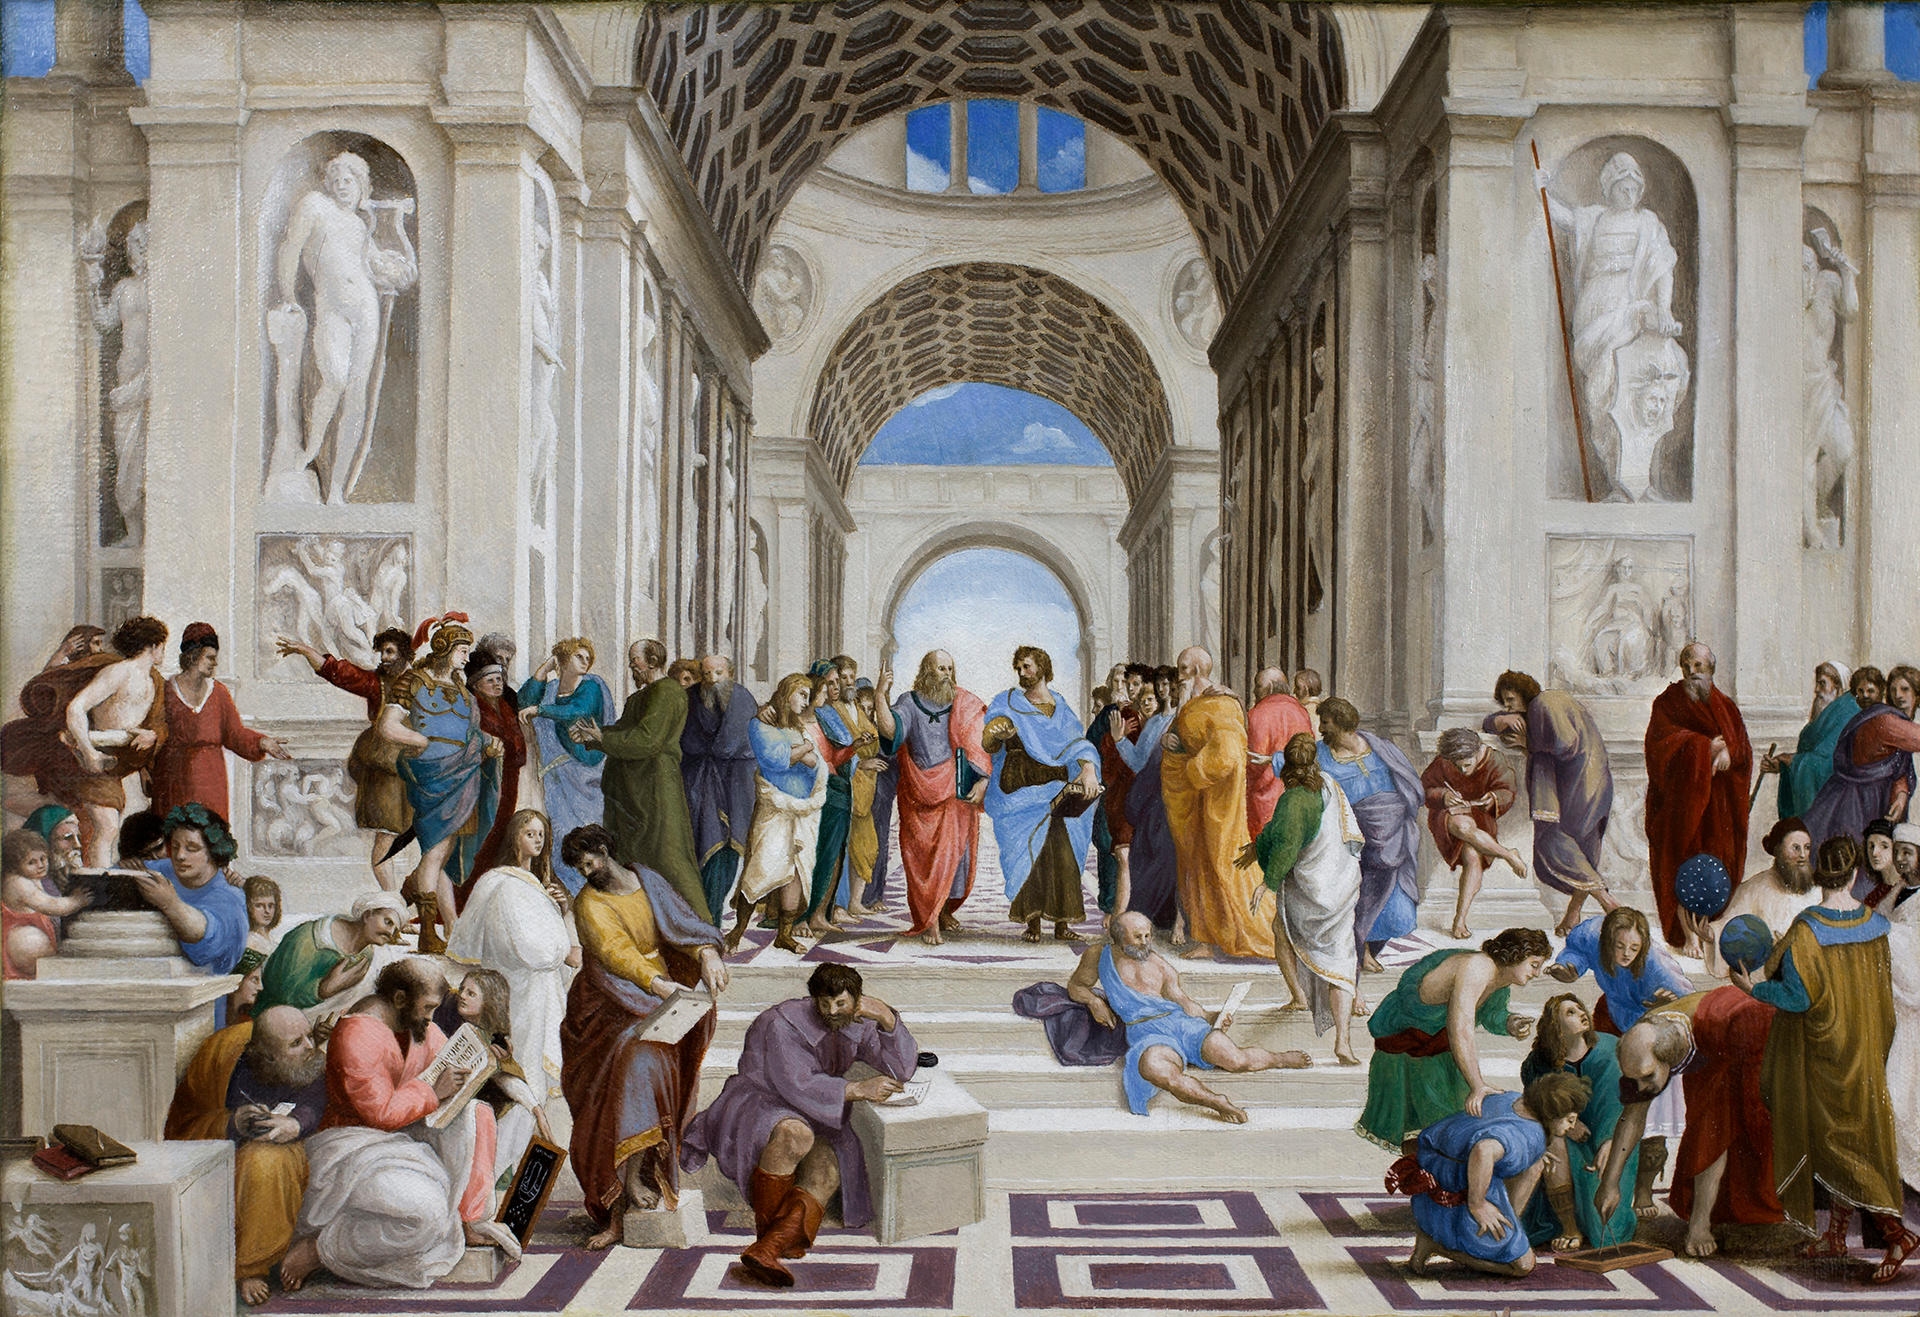
\includegraphics[width=0.9\textwidth]{intro/the_school_of_athens.jpg} % Add an appropriate image to illustrate supplementary and complementary angles
    \end{center}
\end{frame}

\begin{frame}{What is Geometry?}
    \begin{itemize}
        \item Branch of mathematics studying shapes, sizes, and spatial relationships.
        \item Derived from Greek: \textit{"geo"} (earth) + \textit{"metron"} (measure).
        \item Originally focused on measuring the earth, now much broader.
    \end{itemize}
\end{frame}

\begin{frame}{Key Concepts in Geometry}
    \begin{itemize}
        \item \textbf{Points, Lines, and Angles}: Basic building blocks.
        \item \textbf{Shapes and Figures}: Circles, triangles, polygons.
        \item \textbf{Solids}: 3D objects like cubes, spheres, pyramids.
        \item \textbf{Theorems and Proofs}: Logical reasoning based on axioms and postulates.
    \end{itemize}
\end{frame}

\begin{frame}{Why Learning Geometry is Important in ML}
    \begin{itemize}
        \item \textbf{Understanding Data:} ML operates in high-dimensional spaces, where geometry helps analyze structure and relationships.
        \item \textbf{Feature Engineering:} Transformations (rotations, scaling, projections) improve model performance.
        \item \textbf{Distance Metrics:} Algorithms rely on distances (Euclidean, cosine, Manhattan) for clustering and classification.
        \item \textbf{Optimization:} Gradient descent follows geometric paths to minimize loss functions.
        \item \textbf{Manifold Learning:} Real-world data often lies on curved manifolds, requiring non-Euclidean methods (e.g., t-SNE, UMAP).
        \item \textbf{Deep Learning:} CNNs use geometric transformations; GNNs handle graph structures.
        \item \textbf{Model Interpretability:} Decision boundaries (e.g., SVMs) are geometric constructs that explain model behavior.
    \end{itemize}
    \end{frame}


\begin{frame}{Definition of Percentage}
    \begin{itemize}
        \item A \textbf{percentage} is a way of expressing a number as a fraction of 100.
        \item The formula to calculate a percentage is:
    \[
        \text{Percentage} = \left( \frac{\text{Part}}{\text{Whole}} \right) \times 100
    \]
        \item Example: If you score 45 out of 60 on a test, the percentage is:
    \[
        \left( \frac{45}{60} \right) \times 100 = 75\%
    \]
    \end{itemize}
\end{frame}

\begin{frame}
    \frametitle{Ratio vs Rate}
    \begin{figure}[h]    
        \begin{minipage}[b]{0.5\textwidth}
        \centering
        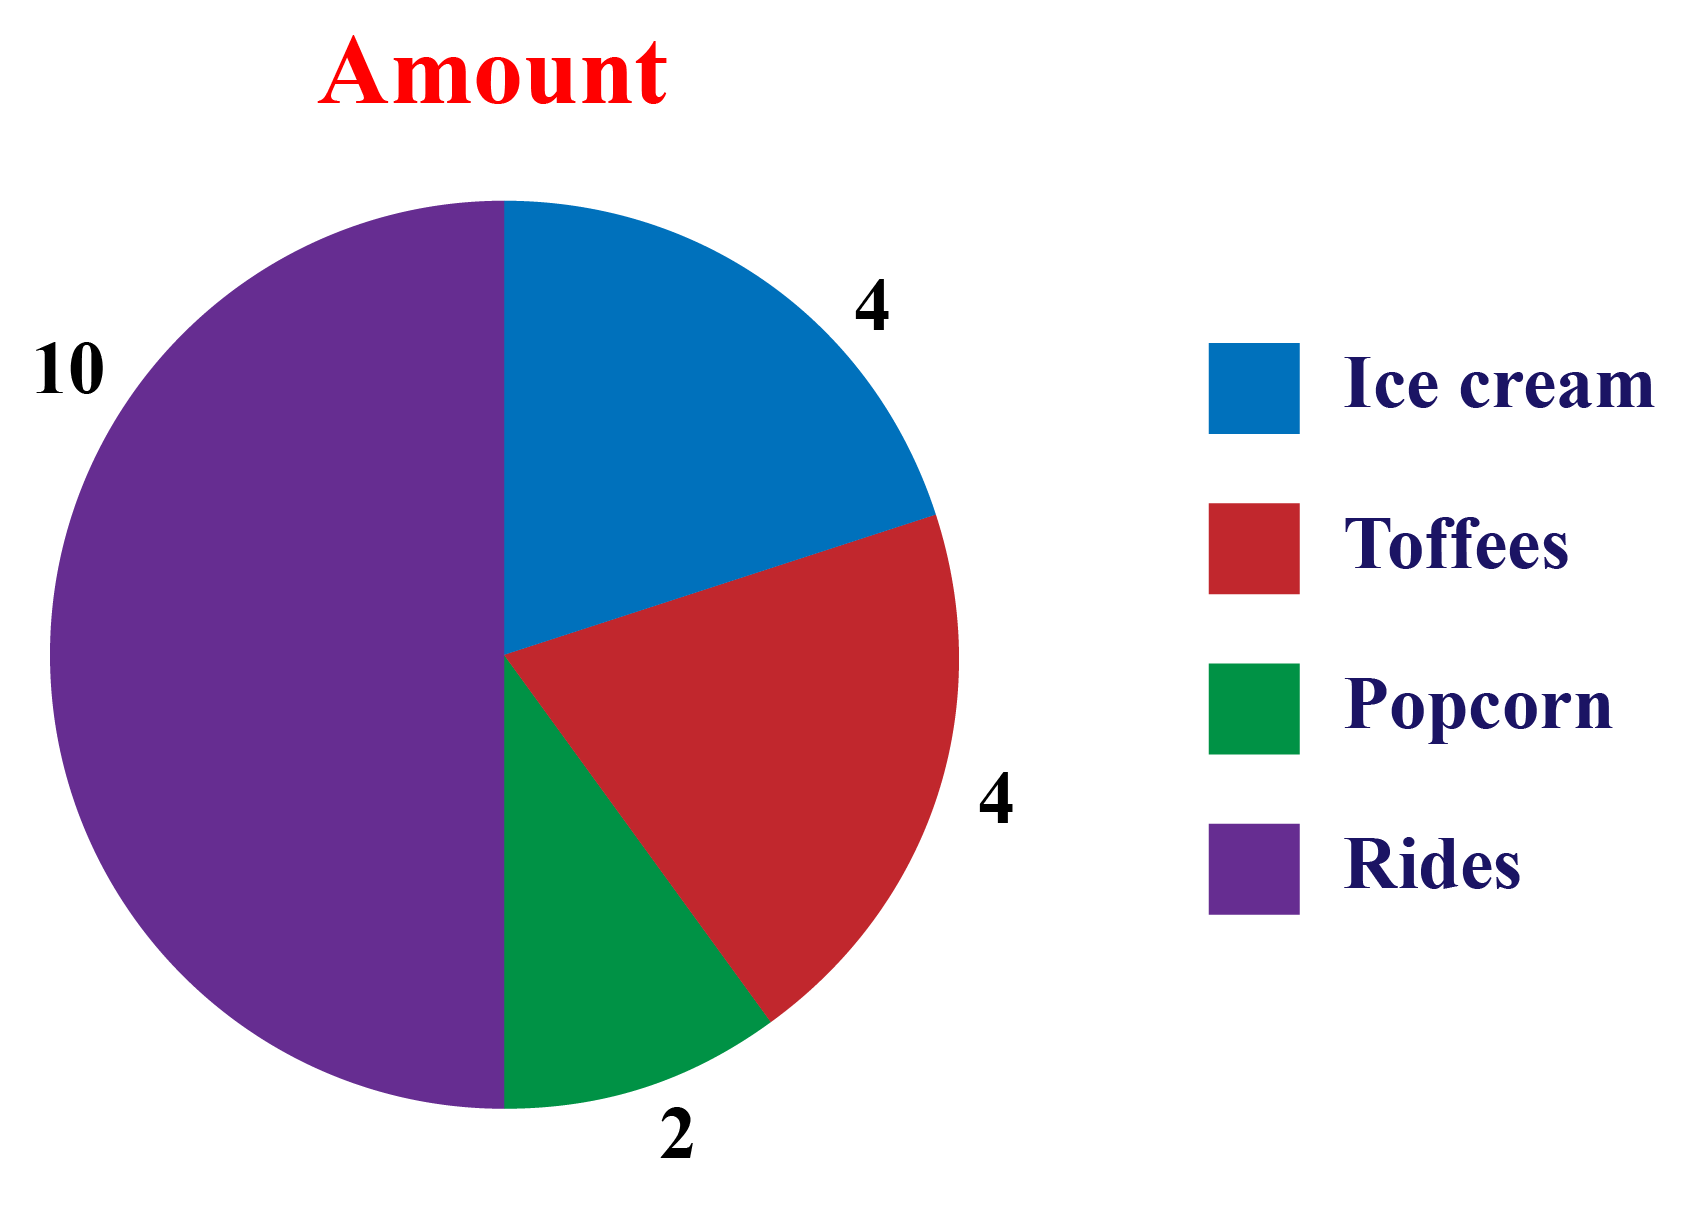
\includegraphics[scale=0.2]{intro/ratio.png}
        \caption{ratio}
    \end{minipage}
    \begin{minipage}[b]{0.4\textwidth}
        \centering
        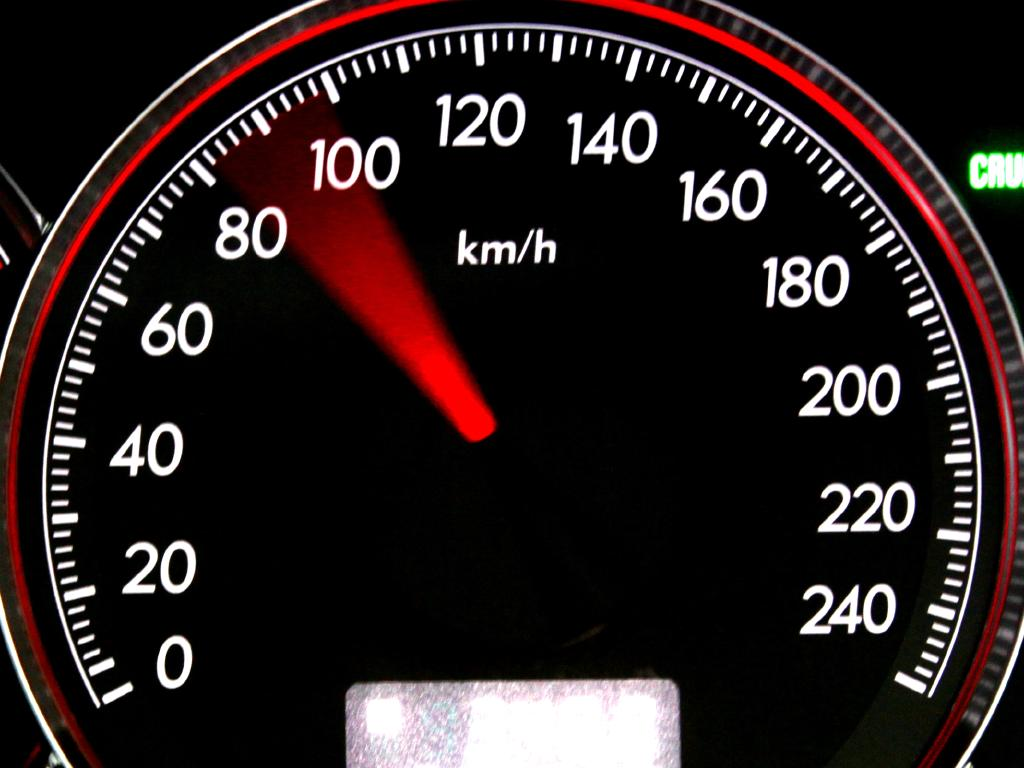
\includegraphics[scale=0.5]{intro/rate.jpeg}
        \caption{rate}
    \end{minipage}
\end{figure}
\end{frame}

\begin{frame}{Key Distinction: Ratio vs Rate}
    \begin{columns}[T] % Split into two columns
        \column{0.5\textwidth}
        \centering
        \textbf{Ratio}
        \begin{itemize}
            \item \textbf{Definition:} Comparison of two similar units.
            \item \textbf{Units:} Unitless (dimensionless).
            \item \textbf{Form:} Written as \( a:b \), \( \frac{a}{b} \), or "a to b".
            \item \textbf{Example:} Boys to girls in a classroom is \( 2:3 \).
            \item \textbf{Key Feature:} Static relationships.
        \end{itemize}

        \column{0.5\textwidth}
        \centering
        \textbf{Rate}
        \begin{itemize}
            \item \textbf{Definition:} Comparison of two different units.
            \item \textbf{Units:} Includes units (e.g., miles per hour).
            \item \textbf{Form:} Written as \( \frac{a \, \text{unit}_1}{b \, \text{unit}_2} \) or "a per b".
            \item \textbf{Example:} A car travels \( 60 \, \text{mph} \).
            \item \textbf{Key Feature:} Dynamic relationships (e.g., over time or space).
        \end{itemize}
    \end{columns}
\end{frame}


\begin{frame}
    \frametitle{Proportional Relationship}

    \begin{block}{Definition}
        A proportional relationship is a relationship between two quantities where the ratio between them remains constant. 
        If two variables are proportional, it means they can be expressed in the form:
        \[ y = kx \]
        where $ k $ is the constant of proportionality and it can be an integer or a fraction or an irrational number.
    \end{block}
\end{frame}

\begin{frame}
    \frametitle{Proportionality Problem: Mixing Chemicals}

    \begin{block}{Problem}
        A person mixes $15 ml$ of bleach with $3.75 L$ of water for sanitizing solution for a daycare. What are the possible combinations 
    \end{block}

    \begin{itemize}
        \item \textbf{A.} 12 mL bleach and 3L water
        \item \textbf{B.} 6 mL bleach and 1.5L water
        \item \textbf{C.} 3 mL leach and 0.75L water
        \item \textbf{D.} 20 mL bleach and 5.5L water
    \end{itemize}
    \begin{block}{Problem}
        Is the area of square is propotional to side length ?
    \end{block}
\end{frame}

\begin{frame}{Proportionality vs. Linearity}
    \begin{itemize}
        \item A \textbf{proportional relationship} always passes through the origin \((0, 0)\).
        \item The general form of a proportional relationship is:
        \[
        y = kx
        \]
        where \(k\) is the constant of proportionality.
        
        \item A \textbf{linear relationship} can pass through any point, not necessarily the origin.
        \item The general form of a linear relationship is:
        \[
        y = mx + b
        \]
        where \(m\) is the slope and \(b\) is the y-intercept.
        
        \item Key Difference:
        \begin{itemize}
            \item In a proportional relationship, \(b = 0\), so the line always passes through \((0, 0)\).
            \item In a linear relationship, \(b\) can be any value, so the line does not need to pass through the origin.
        \end{itemize}
    \end{itemize}
\end{frame}


\begin{frame}{Main Types of Geometry}
    \begin{itemize}
        \item \textbf{Euclidean Geometry}: Deals with flat, 2D spaces.
        \item \textbf{Non-Euclidean Geometry}: Studies curved spaces (spherical, hyperbolic).
        \item \textbf{Analytic Geometry}: Combines algebra and geometry using coordinates.
        \item \textbf{Differential Geometry}: Uses calculus to study curves and surfaces.
    \end{itemize}
\end{frame}

\begin{frame}{Applications of Geometry}
    \begin{itemize}
        \item Essential in fields like architecture, physics, engineering.
        \item Used in navigation, astronomy, and computer graphics.
        \item Provides tools to understand spatial relationships in various disciplines.
    \end{itemize}
\end{frame}

\subsection{Eucledian Geometry} 

\begin{frame}
    \frametitle{Geometry Terminology}
    
    \begin{center}
        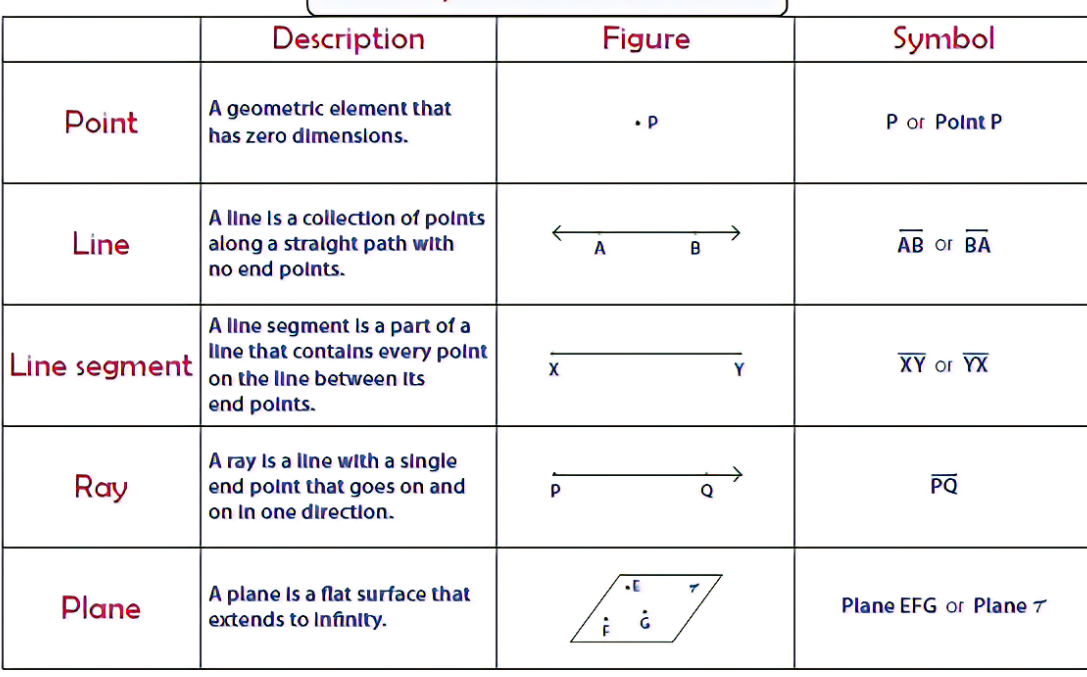
\includegraphics[width=0.8\textwidth]{intro/geometry.png} % Add an appropriate image to illustrate supplementary and complementary angles
    \end{center}
\end{frame}
\begin{frame}
    \frametitle{Geometry Terminology: Coplanar \& Colinear}
    \begin{center}
        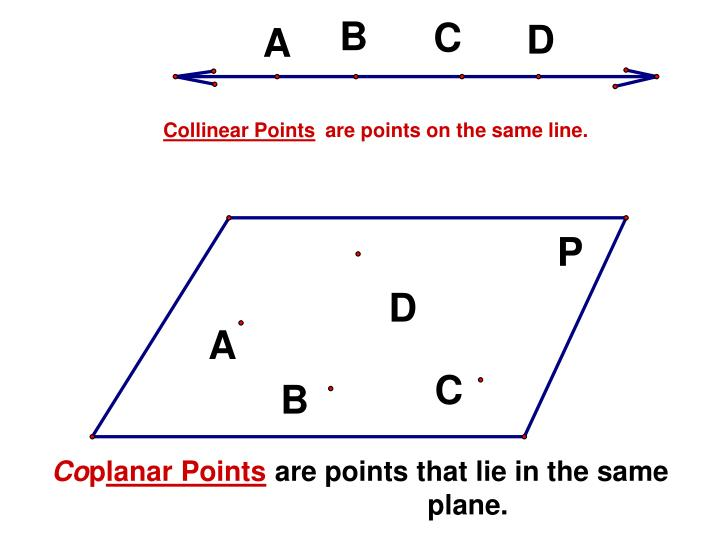
\includegraphics[width=0.8\textwidth]{intro/coplanar.jpg} % Add an appropriate image to illustrate supplementary and complementary angles
    \end{center}
\end{frame}

\begin{frame}
    \frametitle{Geometry Terminology: Dimensions}
    \begin{center}
        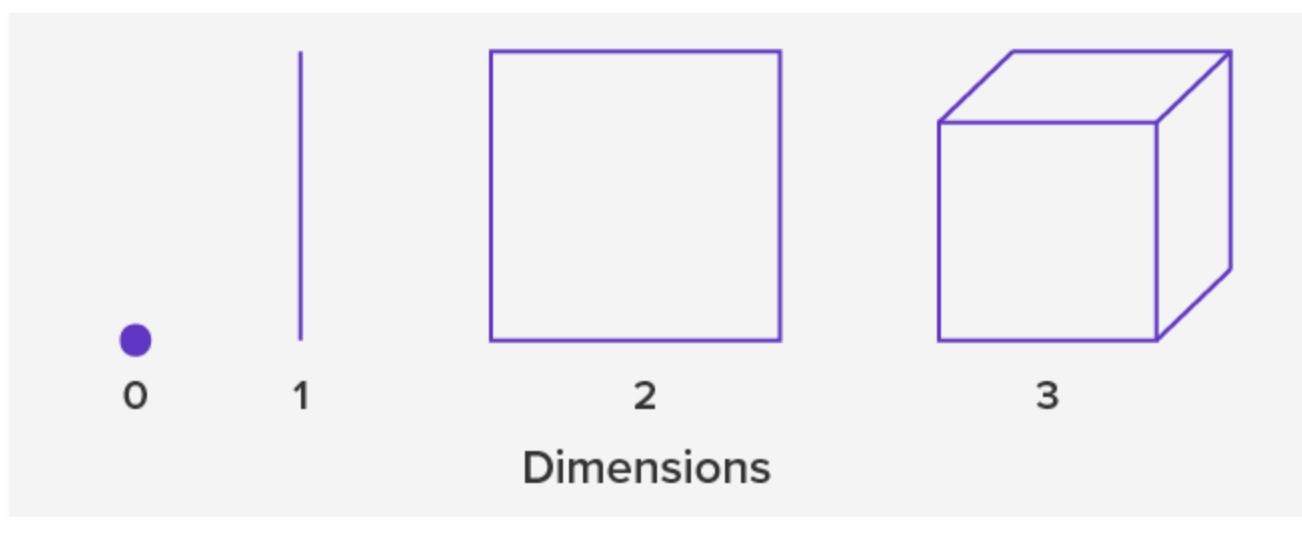
\includegraphics[width=0.8\textwidth]{intro/dimensions.jpeg} % Add an appropriate image to illustrate supplementary and complementary angles
    \end{center}
\end{frame}

\begin{frame}{Parallel \& Perpendicular Lines}
    \begin{block}{Parallel}
      Two lines are said to be \textbf{parallel} if they never intersect, no matter how far they are extended, and remain the same distance apart at all points.
    \end{block}
    \begin{block}{Perpendicular}
        Two lines are said to be \textbf{perpendicular} if they intersect at a right angle (90 degrees).
    \end{block}
  \end{frame}


  \begin{frame}
    \frametitle{Parallel \& Perpendicular Lines}
    \begin{center}
        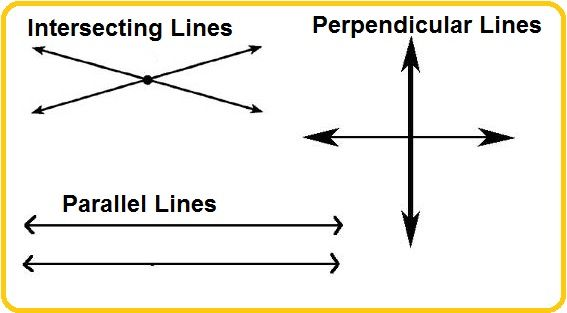
\includegraphics[width=0.8\textwidth]{intro/parallel_perpendicular.jpg} % Add an appropriate image to illustrate supplementary and complementary angles
    \end{center}
\end{frame}




\begin{frame}{Angles}
    \begin{itemize}
        \item \textbf{Angle}: Formed by two rays with a common endpoint.
        \item \textbf{Acute Angle}: Less than 90°.
        \item \textbf{Right Angle}: Exactly 90°.
        \item \textbf{Obtuse Angle}: Greater than 90° but less than 180°.
        \item \textbf{Straight Angle}: Exactly 180°.
    \end{itemize}
\end{frame}

\begin{frame}{Shapes and Figures}
    \begin{itemize}
        \item \textbf{Polygon}: A closed figure formed by line segments.
        \item \textbf{Triangle}: A polygon with three sides.
        \begin{itemize}
            \item \textbf{Equilateral Triangle}: All sides and angles are equal.
            \item \textbf{Isosceles Triangle}: Two sides and angles are equal.
            \item \textbf{Scalene Triangle}: All sides and angles are different.
        \end{itemize}
        \item \textbf{Quadrilateral}: A polygon with four sides (e.g., square, rectangle).
        \item \textbf{Circle}: A set of points equidistant from the center.
    \end{itemize}
\end{frame}

\begin{frame}{Properties of Shapes}
    \begin{itemize}
        \item \textbf{Perimeter}: Total distance around a shape.
        \item \textbf{Area}: The measure of space inside a two-dimensional shape.
        \item \textbf{Volume}: The measure of space inside a three-dimensional object.
    \end{itemize}
\end{frame}

\begin{frame}{Transformations}
    \begin{itemize}
        \item \textbf{Translation}: Moving a shape without rotating or flipping it.
        \item \textbf{Rotation}: Turning a shape around a fixed point.
        \item \textbf{Reflection}: Flipping a shape over a line to create a mirror image.
        \item \textbf{Dilation}: Resizing a shape while maintaining its proportions.
    \end{itemize}
\end{frame}

\begin{frame}
    \frametitle{Parallel Lines}
    
    \begin{itemize}
        \item \textbf{Definition:} Two or more lines that are always the same distance apart and never meet, no matter how far they are extended.
        \item They run in the same direction and have the same slope.
        \item Example: Think of train tracks running side by side—they never cross each other.
    \end{itemize}
    
    \begin{center}
        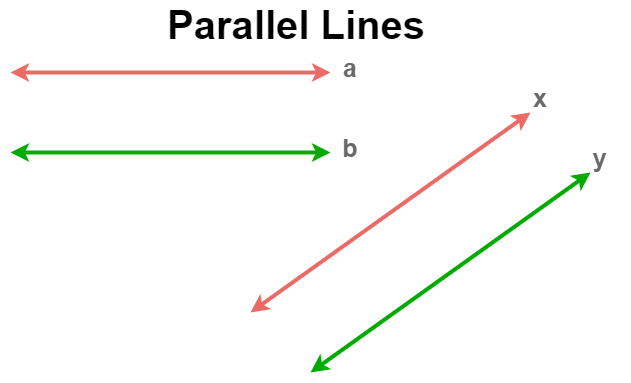
\includegraphics[width=0.5\textwidth]{intro/Parallellines.png} % Add an appropriate image to illustrate parallel lines
    \end{center}

\end{frame}
\begin{frame}
    \frametitle{Angles}
\end{frame}

\begin{frame}
    \frametitle{Supplementary and Complementary Angles}
       
    \begin{center}
        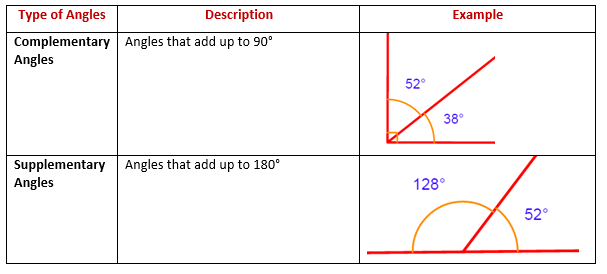
\includegraphics[width=0.9\textwidth]{intro/complementary_supplementary_angles.png} % Add an appropriate image to illustrate supplementary and complementary angles
    \end{center}

\end{frame}

\begin{frame}
    \frametitle{Problem 1}
    
    \begin{center}
        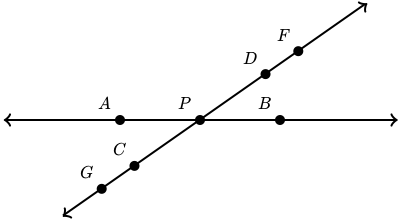
\includegraphics[width=0.9\textwidth]{intro/supplementary_angles.png} % Add an appropriate image to illustrate supplementary and complementary angles
    \end{center}

\end{frame} 

\begin{frame}
    \frametitle{Vertical Angles}
    \begin{block}{}
        Vertical angles, also known as opposite angles, are the angles formed when two lines intersect
    \end{block}
    \begin{center}
        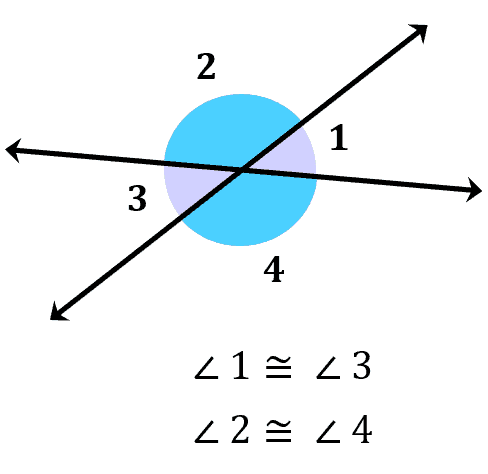
\includegraphics[width=0.5\textwidth]{intro/vertical_angles_1.png} % Add an appropriate image to illustrate supplementary and complementary angles
    \end{center}

\end{frame}


\begin{frame}
    \frametitle{Problem 2: Vertical Angles}
\begin{center}
    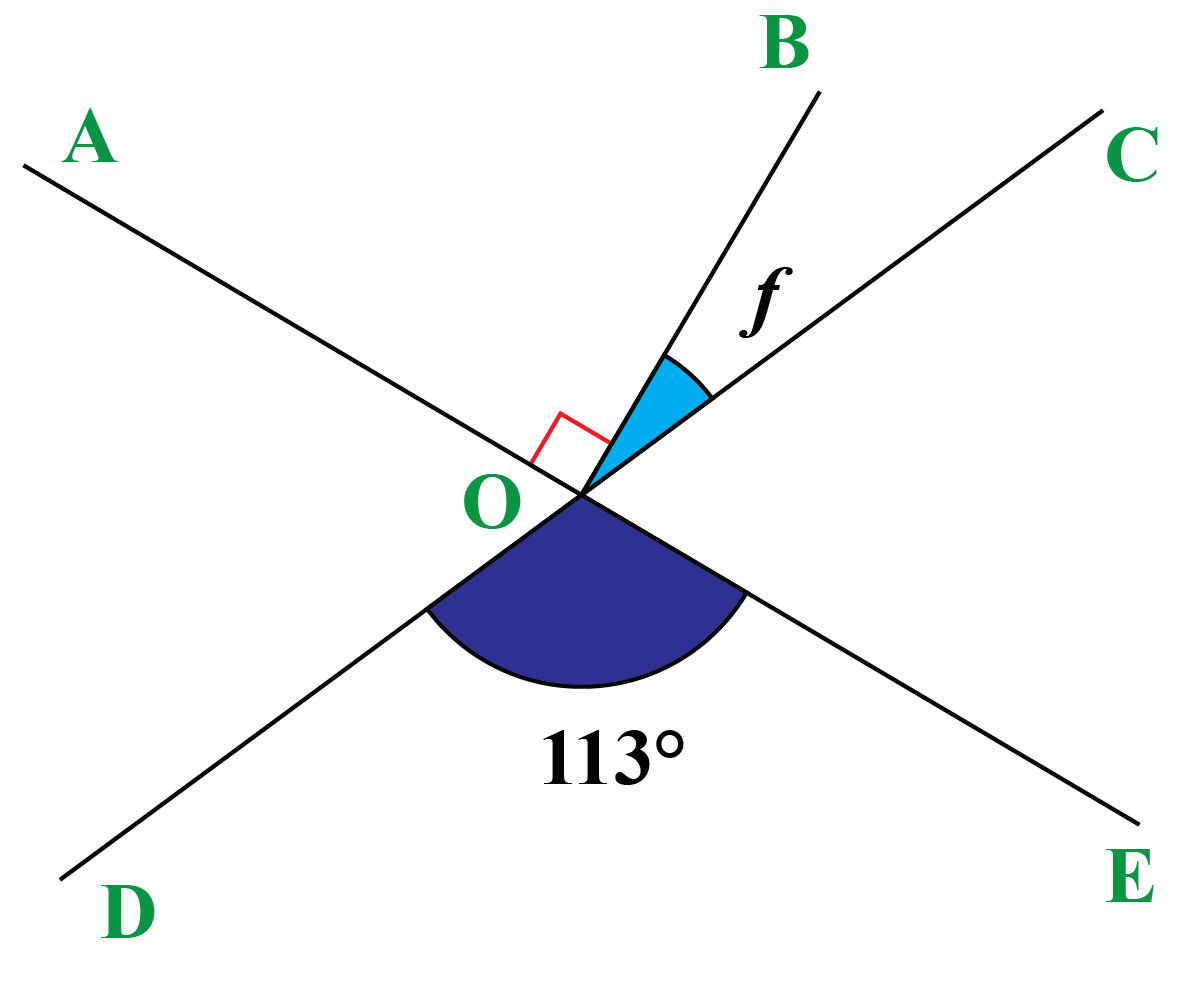
\includegraphics[width=0.5\textwidth]{intro/vertical_angles_2.png} % Add an appropriate image to illustrate supplementary and complementary angles
\end{center}
\end{frame}


\begin{frame}{Transversal \& Parallel Lines}
    A \textbf{transversal line} is a line that crosses or intersects two or more other lines at different points
    \begin{figure}[h]    
        \begin{minipage}[b]{0.4\textwidth}
        \centering
        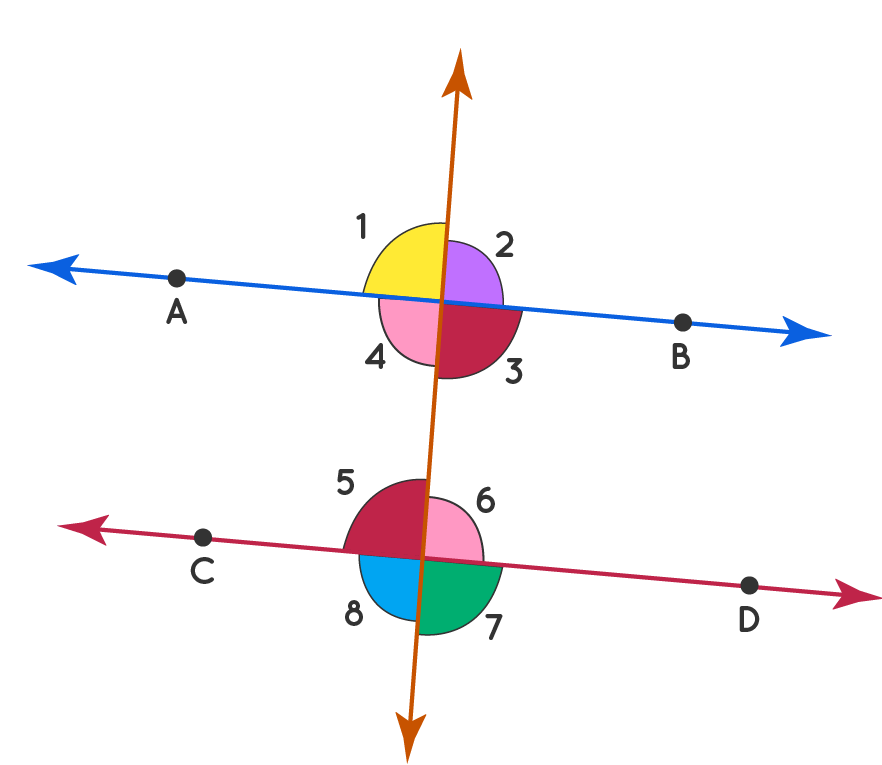
\includegraphics[scale=0.15]{intro/alternate_interior_angles.png}
        \caption{alternate interior angles}
    \end{minipage}
    \begin{minipage}[b]{0.4\textwidth}
        \centering
        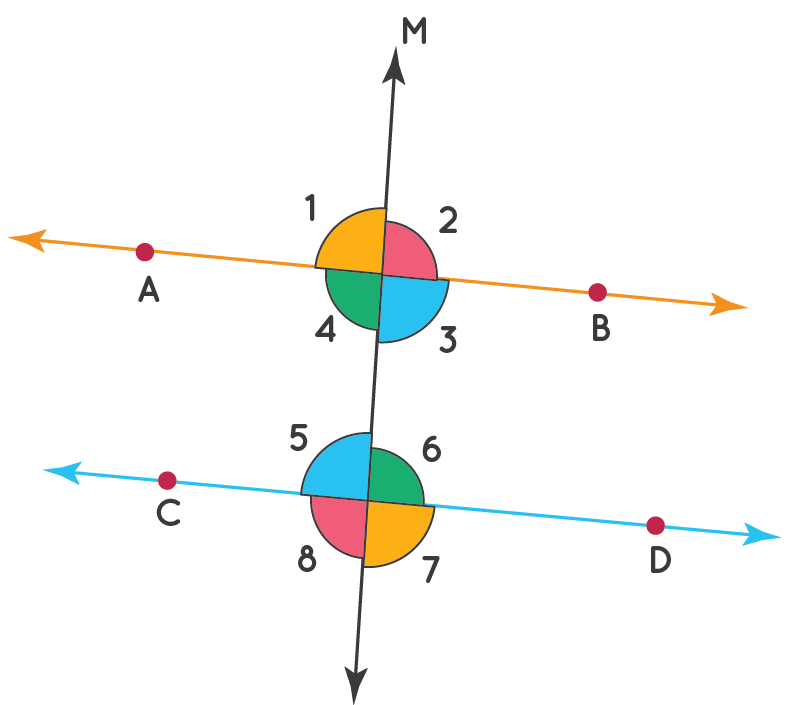
\includegraphics[scale=0.15]{intro/alternate_exterior_angles.png}
        \caption{alternate exterior angles}
    \end{minipage}
\end{figure}
    
\end{frame}




\begin{frame}
    \frametitle{Altitudes, Medians and Centroid} 

    \begin{figure}[h]    
        \begin{minipage}[b]{0.4\textwidth}
        \centering
        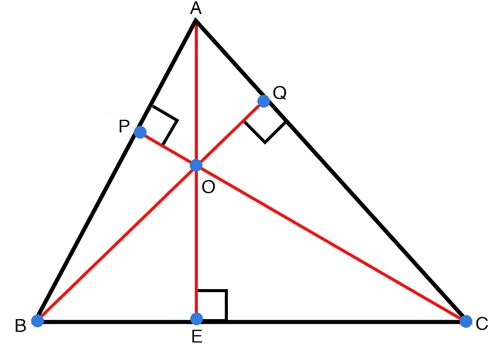
\includegraphics[scale=0.25]{intro/altitudes.jpeg}
        \caption{altitudes}
    \end{minipage}
    \begin{minipage}[b]{0.4\textwidth}
        \centering
        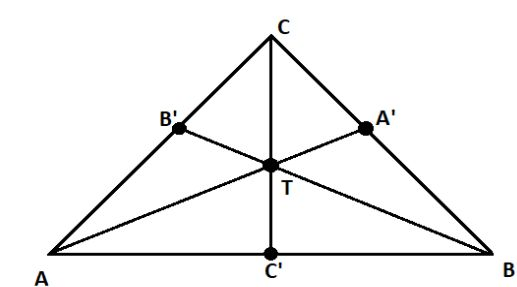
\includegraphics[scale=0.25]{intro/medians.jpeg}
        \caption{medians}
    \end{minipage}
\end{figure}
\end{frame}

\begin{frame}
    \frametitle{Exterior Angle Property}
    \begin{center}
        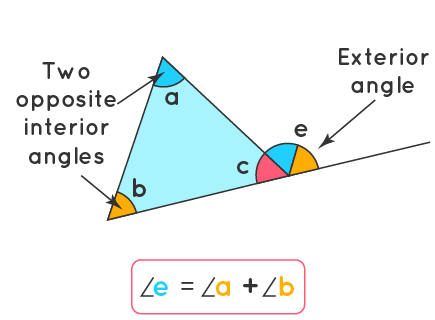
\includegraphics[width=0.5\textwidth]{intro/exterior_angle.png} 
    \end{center}
\end{frame}

\begin{frame}
    \frametitle{Angles of a Triangle Measure to $180^\circ$}
    \begin{center}
        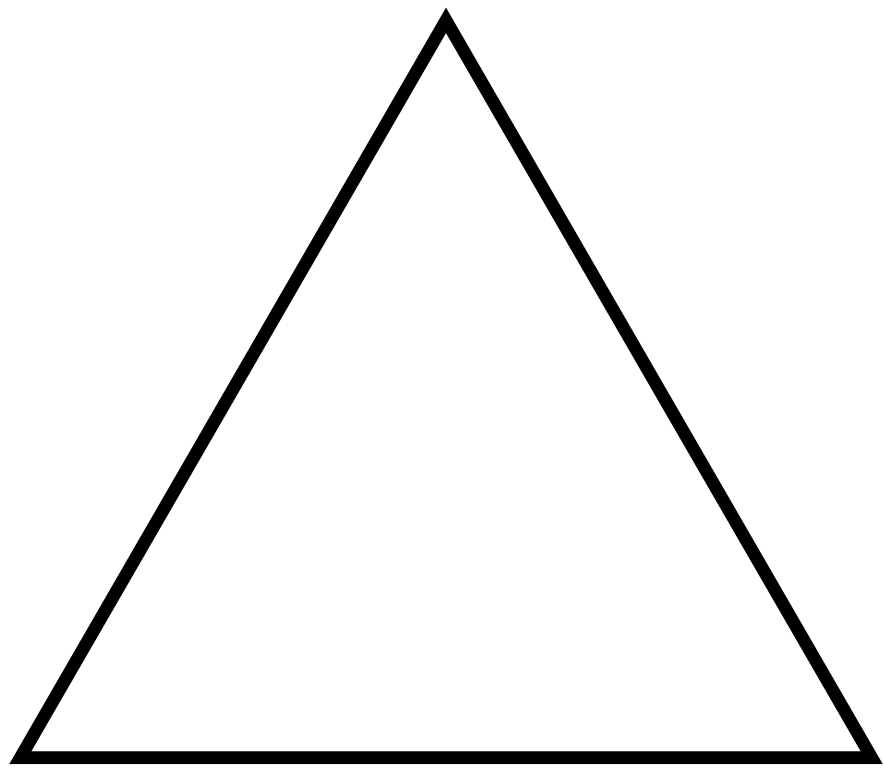
\includegraphics[width=0.5\textwidth]{intro/triangle.png} 
    \end{center}
\end{frame}

\begin{frame}
    \frametitle{Equilateral and Isosceles Triangle}
    \begin{figure}[h]    
        \begin{minipage}[b]{0.4\textwidth}
        \centering
        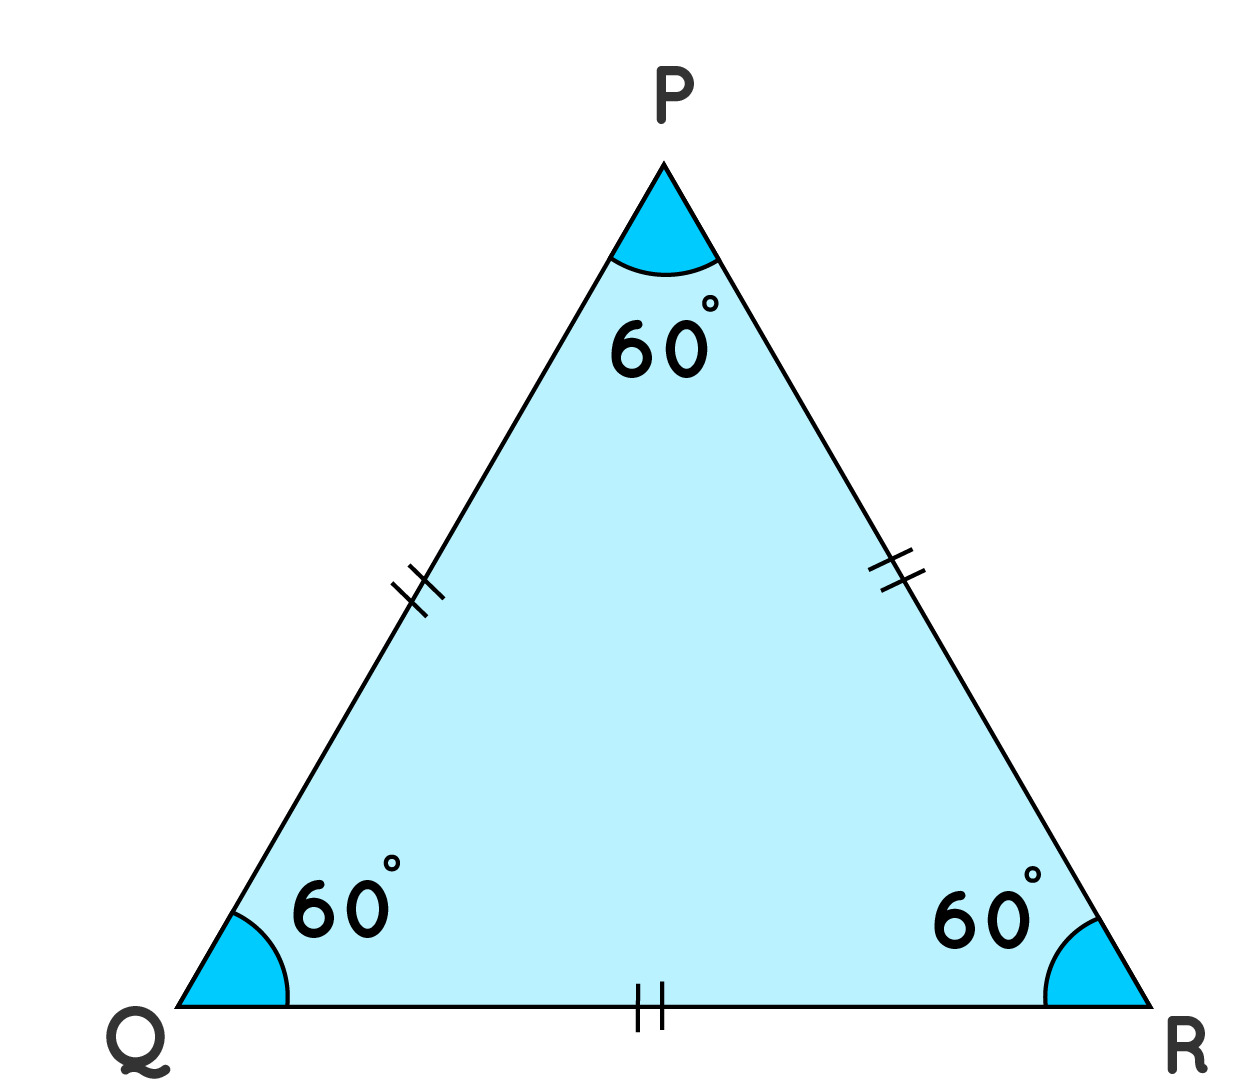
\includegraphics[scale=0.1]{intro/equilateral_triangle.png}
        \caption{Equilateral}
    \end{minipage}
    \begin{minipage}[b]{0.4\textwidth}
        \centering
        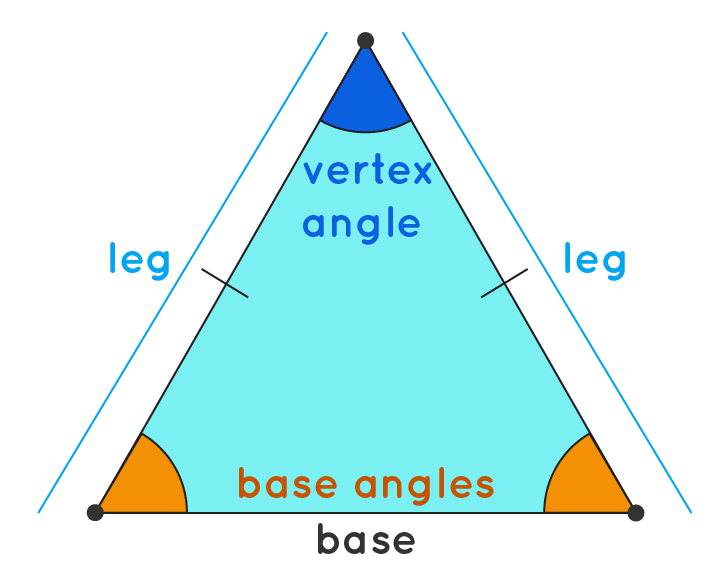
\includegraphics[scale=0.15]{intro/isoscles_triangle.png}
        \caption{Isosceles}
    \end{minipage}
\end{figure}
\end{frame}

\begin{frame}
    \frametitle{Triangle Inequality}
    \begin{block}{}
        For any triangle with sides \(a\), \(b\), and \(c\), the following conditions must hold true:
         \begin{itemize}
                \item \( a + b > c \)
                \item \( a + c > b \)
                \item \( b + c > a \)
        \end{itemize}
    \end{block}
    \begin{center}
        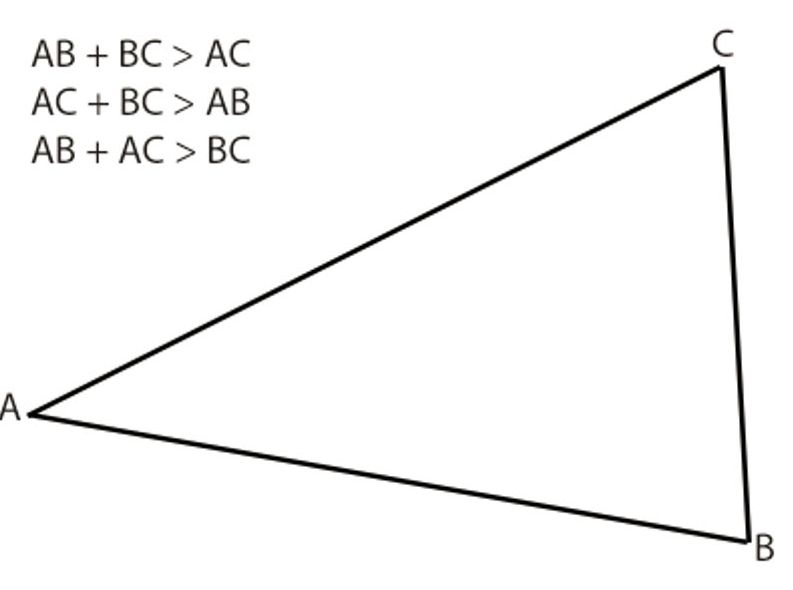
\includegraphics[width=0.3\textwidth]{intro/triangle_inequality.jpeg} 
    \end{center}
\end{frame}

\section{Similarity}

\subsection{Transformations}



    
    % Slide: Introduction
    \begin{frame}{What are Rigid Transformations?}
        \begin{itemize}
            \item Rigid transformations (or isometries) preserve the shape and size of geometric objects.
            \item They do not alter:
            \begin{itemize}
                \item Distances between points.
                \item Angles between lines or curves.
            \end{itemize}
            \item The object remains congruent to itself after the transformation.
        \end{itemize}
    \end{frame}
    
    % Slide: Types of Rigid Transformations
    \begin{frame}{Types of Rigid Transformations}
        \begin{enumerate}
            \item \textbf{Translation:} Moves every point by the same distance in a given direction.
            \item \textbf{Rotation:} Rotates an object around a fixed point by a certain angle.
            \item \textbf{Reflection:} Flips an object over a specified line (the "mirror line").
            \item \textbf{Glide Reflection:} Combines a reflection and a translation along the direction of the reflection line.
        \end{enumerate}
    \end{frame}
    
    % Slide: Translation
    \begin{frame}{Translation}
        \textbf{Definition:}
        \begin{itemize}
            \item Moves every point of an object by the same distance in a specific direction.
        \end{itemize}
        \textbf{Mathematical Representation:}
        \[
        (x', y') = (x + a, y + b)
        \]
        \textbf{Properties:}
        \begin{itemize}
            \item Preserves distances and angles.
            \item Does not change the orientation of the object.
        \end{itemize}
    \end{frame}
    
    % Slide: Rotation
    \begin{frame}{Rotation}
        \textbf{Definition:}
        \begin{itemize}
            \item Rotates an object around a fixed point by a certain angle.
        \end{itemize}
        \textbf{Mathematical Representation:}
        For a rotation by angle \(\theta\) around the origin:
        \[
        x' = x \cos\theta - y \sin\theta
        \]
        \[
        y' = x \sin\theta + y \cos\theta
        \]
        \textbf{Properties:}
        \begin{itemize}
            \item Preserves distances and angles.
            \item Changes the orientation depending on the direction of rotation.
        \end{itemize}
    \end{frame}
    
    % Slide: Reflection
    \begin{frame}{Reflection}
        \textbf{Definition:}
        \begin{itemize}
            \item Flips an object over a line (the "mirror line").
        \end{itemize}
        \textbf{Examples:}
        \begin{itemize}
            \item Reflection across the \(x\)-axis, \(y\)-axis, or any line \(y = mx + c\).
        \end{itemize}
        \textbf{Properties:}
        \begin{itemize}
            \item Preserves distances and angles.
            \item Changes the orientation of the object.
        \end{itemize}
    \end{frame}
    
    % Slide: Properties of Rigid Transformations
    \begin{frame}{Properties of Rigid Transformations}
        \begin{itemize}
            \item \textbf{Distance Preservation:} The distance between any two points remains unchanged.
            \item \textbf{Angle Preservation:} Angles between lines or curves are preserved.
            \item \textbf{Parallelism:} Parallel lines remain parallel.
            \item \textbf{Co-ordinates} Co-ordinates ae not preserved 
            \item \textbf{Congruence:} The original and transformed shapes are congruent.
        \end{itemize}
    \end{frame}
    
  \begin{frame}
    \frametitle{Exercise: Rigid Transformations}
    \begin{center}
        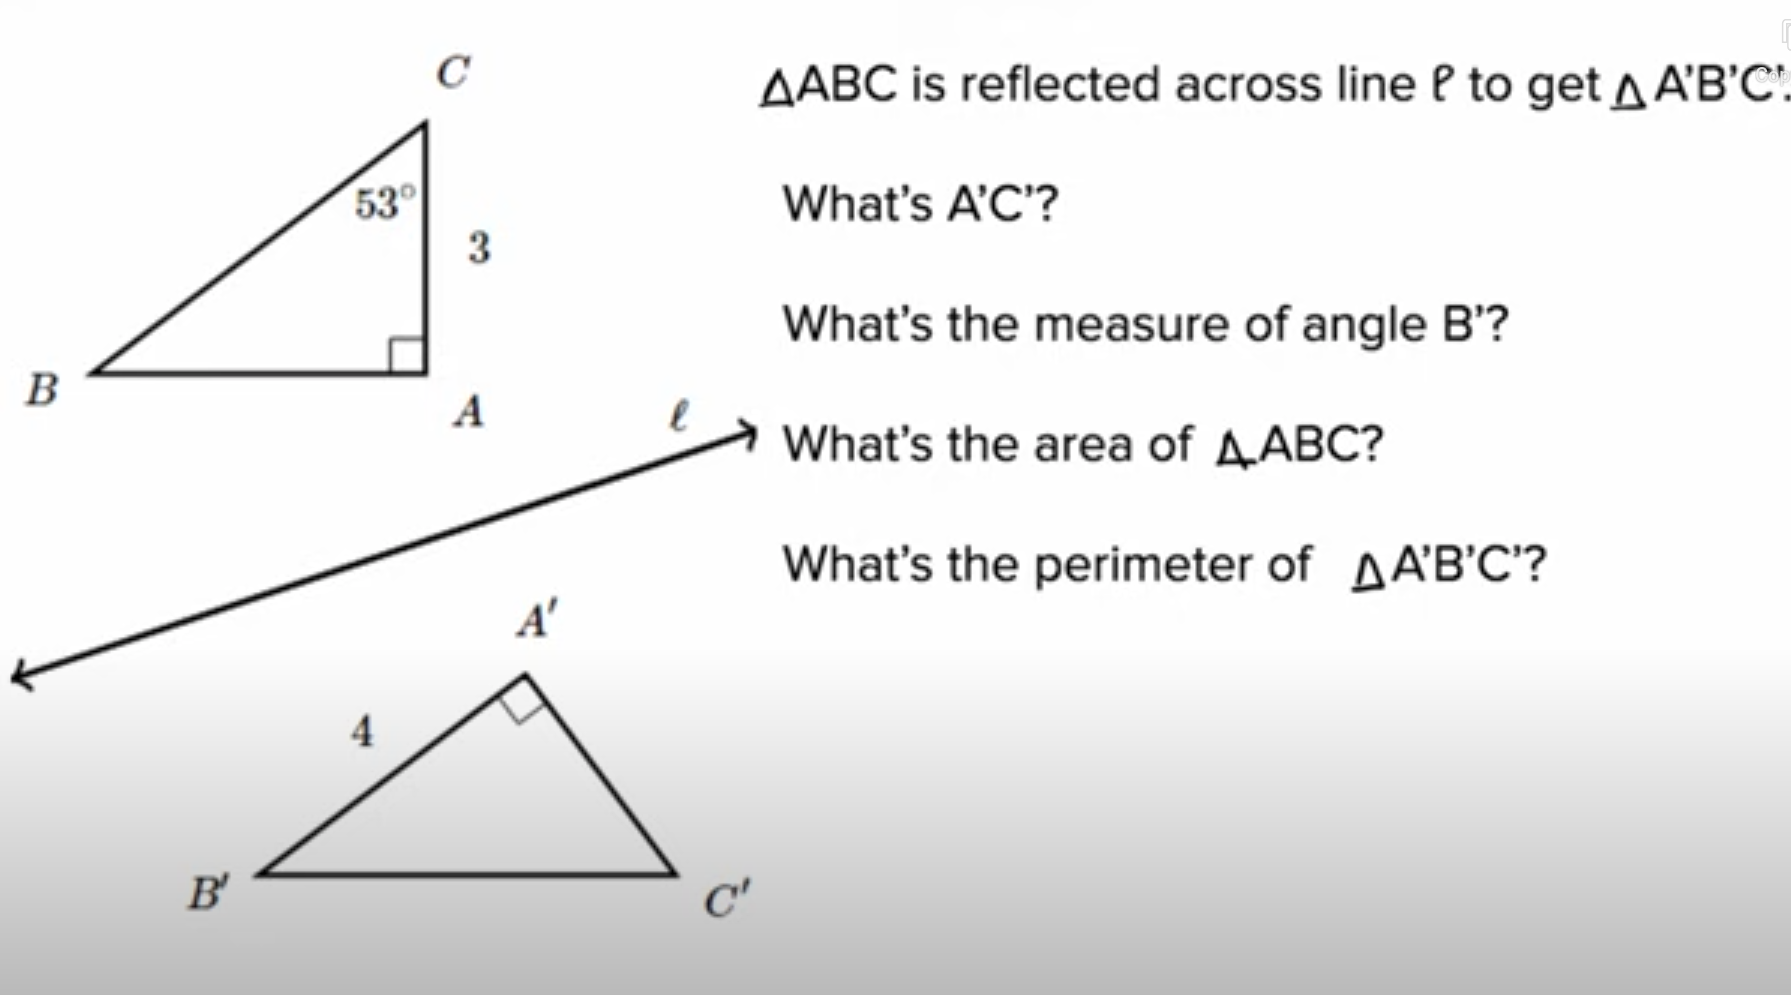
\includegraphics[width=0.9\textwidth]{intro/exer_20.png} 
    \end{center}
  \end{frame}

  \begin{frame}
    \frametitle{Dilations}
    \textbf{Definition:}
        \begin{itemize}
            \item Dilation involves scaling distances from a point (the center of dilation) by a constant factor $k$. It changes the size of a figure but not its shape.
        \end{itemize}
    \begin{itemize}
        \item A non rigid transformation where lengths are not preserved 
        \item Dilation will preserve angles 
    \end{itemize}
\end{frame}
    \subsection{Congruence}
    \begin{frame}
        \frametitle{What is Congruence}
        \begin{block}{Definition}
            Congruence means that two figures or shapes are identical in shape and size. 
            They can be transformed into each other using rigid transformations such as translation, rotation, or reflection 
        \end{block}

        \begin{itemize}
            \item Vertical angles are congruent
            \item Alternate interior angles are congruent
            \item Alternate exterior angles are congruent
            \item Corresponding angles are congruent
        \end{itemize}
    \end{frame}

    \subsection{Congruence in Triangles}
    \begin{frame}
        \frametitle{Congruence in Triangles}
        \begin{block}{SSS}
            if three sides of one triangle are congruent to the three sides of another triangle
        \end{block}
        \begin{block}{SAS}
            if two sides and an included angle of one triangle is congruent to another
        \end{block}
        \begin{block}{ASA}
            if two angles and included side of a triangle is  congruent to another 
        \end{block}
        \begin{block}{AAS}
            if two angles and non included side of a triangle is congruent to another 
        \end{block}
    \end{frame}

     \subsection{Similarity in Triangles}
        \begin{frame}
            \frametitle{Similarity in Triangles}
            \begin{block}{AAA}
                if three angles of one triangle are congruent to another 
            \end{block}
            \begin{block}{SSS}
                if three sides of a triangle are proportional to another
            \end{block}
            \begin{block}{SAS}
                if two sides of a triangle are proportional and included angle is congruent 
            \end{block}
        \end{frame}

\begin{frame}
    \frametitle{What is a Unit Circle}
    \begin{block}{The Unit circle}
        The unit circle is the circle with radius 1 centered at the origin 
    \end{block}
    \begin{block}{Equation of unit Circle}
        The unit circle in the xy-plane is the set of points (x,y) such that
        $$x^{2} + y^{2} = 1$$
        
    \end{block}
    
    \end{frame}
    
    \begin{frame}
    \frametitle{Radius corresponding to a positive angle}
    \centering
    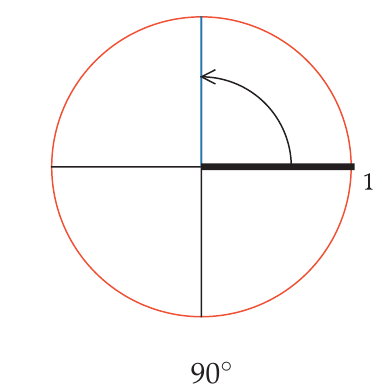
\includegraphics[scale=0.5]{intro/1.png}    \end{frame}
    
    \begin{frame}
    \frametitle{Radius corresponding to a negative angle}
    \centering
    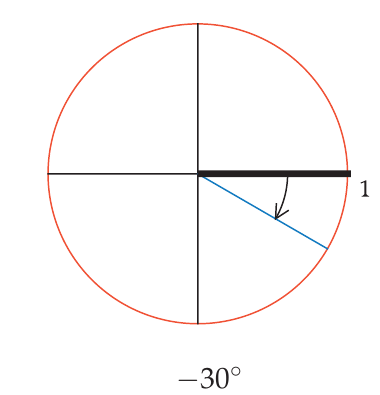
\includegraphics[scale=0.5]{intro/2.png}    \end{frame}
    
    \begin{frame}
        \begin{block}{Positive and Negative Angles}
            \begin{itemize}
                \item Angle measurements for a radius on the unit circle are made from the
                positive horizontal axis.
                \item Positive angles correspond to moving counterclockwise from the positive
                horizontal axis.
                \item Negative angles correspond to moving clockwise from the positive hori-
                zontal axis.
            \end{itemize}
        \end{block}
    \end{frame}
    
    \begin{frame}
        \begin{figure}[h]    
            \begin{minipage}[b]{0.3\textwidth}
            \centering
            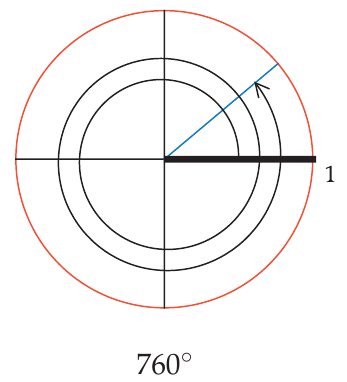
\includegraphics[scale=0.25]{intro/3.png}
            \caption{+ve angle}
        \end{minipage}
        \begin{minipage}[b]{0.3\textwidth}
            \centering
            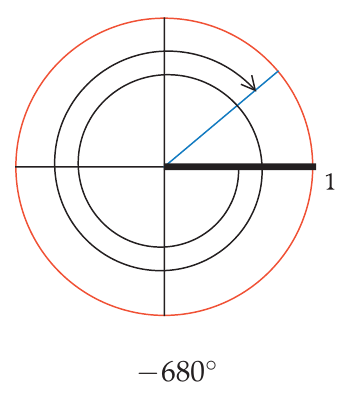
\includegraphics[scale=0.25]{intro/4.png}
            \caption{-ve angle}
        \end{minipage}
    \end{figure}
    \begin{block}{cyclic hehaviour of angles}
        A radius of the unit circle corresponding to $\theta$ degrees also corresponds to
    $\theta + 360n$ degrees for every integer n.
    \end{block}
    \end{frame}
    
    
    \begin{frame}
        \frametitle{Length of a Circular Arc}
        \centering
        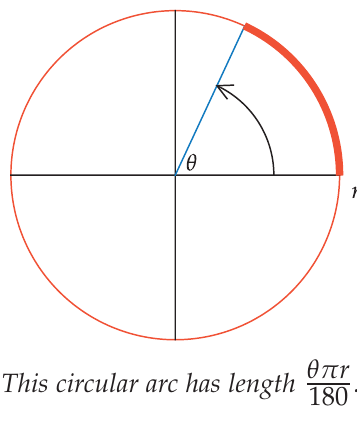
\includegraphics[scale=0.5]{intro/5.png}
    \end{frame}
    
    \begin{frame}
        \frametitle{Radians}
       \begin{block}{Radians}
        Radians are a unit of measurement for angles such that $2\pi$ radians correspond
        to a rotation through an entire circle.
       \end{block}
    \end{frame}
    
    \begin{frame}
        \frametitle{Radians}
        \centering
        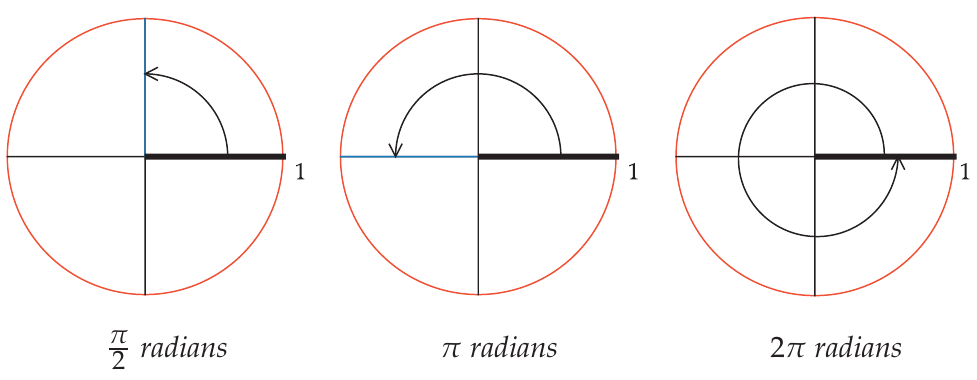
\includegraphics[scale=0.3]{intro/6.png}
    \end{frame}
    \begin{frame}
        \frametitle{Radians}
       \begin{block}{Degree to Radians}
    
        $$ 360^{\circ} = 2 \pi radians $$
        $$ 1 ^{\circ}  = \frac{2 \pi}{360} radians $$
        
       \end{block}
    \end{frame}
    
    \begin{frame}
        \frametitle{Arc Length}
        \begin{block}{length of a circular arc}
            If $0 < \theta \leq 2\pi$ , then a circular arc on the unit circle corresponding to $\theta$ radians
            has length $\theta$         
        \end{block}
    \end{frame}
    
    \begin{frame}
            \begin{figure}[h]    
                \begin{minipage}[b]{0.3\textwidth}
                \centering
                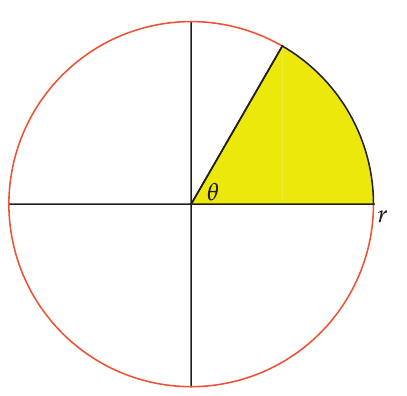
\includegraphics[scale=0.25]{intro/7.png}
                \caption{Area of slice}
            \end{minipage}
        \end{figure}
        \begin{block}{Area of slice}
            A slice with angle $\theta$ radians inside a circle with radius $r$ has area $\frac{1}{2} \theta r^{2}$ .
        \end{block}
    \end{frame}
    
    \begin{frame}
        \frametitle{Cosine and Sine}
        \begin{figure}[h]    
            \begin{minipage}[b]{0.8\textwidth}
            \centering
            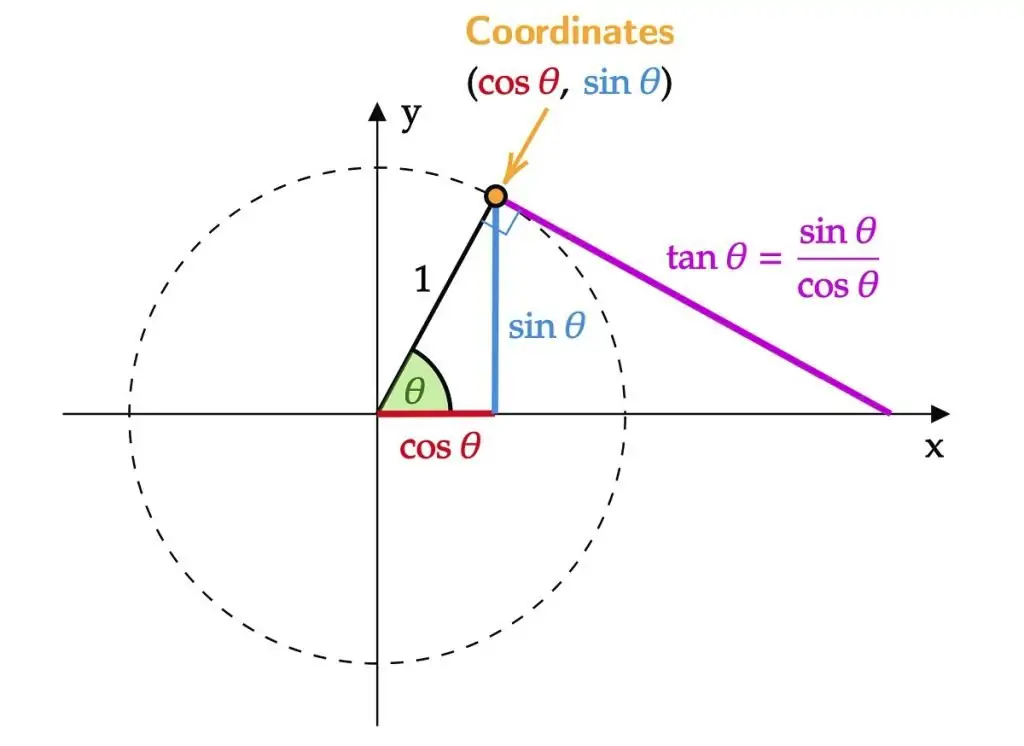
\includegraphics[scale=0.22]{intro/8.png}
            \caption{sin and cos}
        \end{minipage}
    \end{figure}
    \end{frame}


\section{Statistics}
\begin{frame}
    \frametitle{Variability}
    \begin{block}{Variability}
        Variability refers to how data points differ from one another within a data set. In real-world data, there is almost always some variation because no two measurements, observations, or events are exactly the same.
    \end{block}
\end{frame}

\begin{frame}
    \frametitle{Variability Problems}
        \begin{itemize}
            \item How much does my pet weight ?
            \item What is the average number of cars in a parking lot on Monday mornings ?
            \item Am i hungry?
            \item How often am I hungry after lunch ? 
            \item How much time do you spend on facebook every month? 
        \end{itemize}
\end{frame}


\begin{frame}
    \frametitle{Radius corresponding to a positive angle}
    \centering
    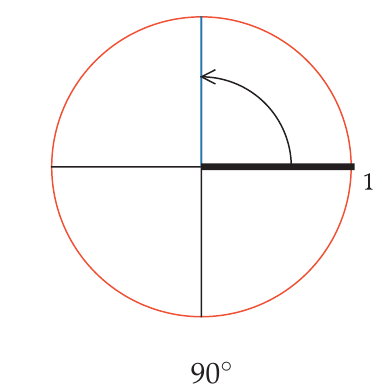
\includegraphics[scale=0.5]{intro/1.png}

\end{frame}

\begin{frame}
    \frametitle{Radius corresponding to a negative angle}
    \centering
    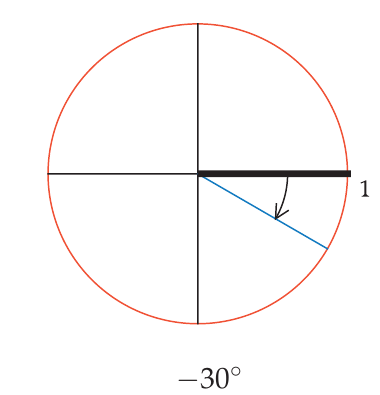
\includegraphics[scale=0.5]{intro/2.png}

\end{frame}

\begin{frame}
    \begin{block}{Positive and Negative Angles}
        \begin{itemize}
            \item Angle measurements for a radius on the unit circle are made from the
            positive horizontal axis.
            \item Positive angles correspond to moving counterclockwise from the positive
            horizontal axis.
            \item Negative angles correspond to moving clockwise from the positive hori-
            zontal axis.
        \end{itemize}
    \end{block}
\end{frame}

\begin{frame}
    \begin{figure}[h]    
        \begin{minipage}[b]{0.3\textwidth}
        \centering
        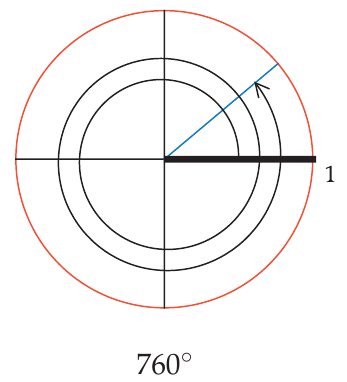
\includegraphics[scale=0.25]{intro/3.png}
        \caption{+ve angle}
    \end{minipage}
    \begin{minipage}[b]{0.3\textwidth}
        \centering
        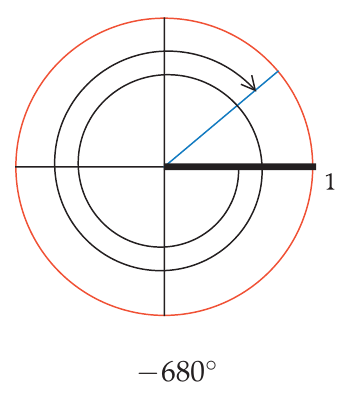
\includegraphics[scale=0.25]{intro/4.png}
        \caption{-ve angle}
    \end{minipage}
\end{figure}
\begin{block}{cyclic hehaviour of angles}
    A radius of the unit circle corresponding to $\theta$ degrees also corresponds to
$\theta + 360n$ degrees for every integer n.
\end{block}
\end{frame}


\begin{frame}
    \frametitle{Length of a Circular Arc}
    \centering
    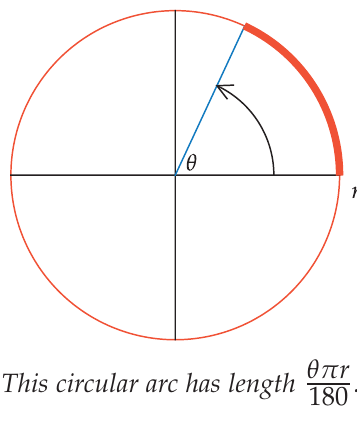
\includegraphics[scale=0.5]{intro/5.png}
\end{frame}

\begin{frame}
    \frametitle{Radians}
   \begin{block}{Radians}
    Radians are a unit of measurement for angles such that $2\pi$ radians correspond
    to a rotation through an entire circle.
   \end{block}
\end{frame}

\begin{frame}
    \frametitle{Radians}
    \centering
    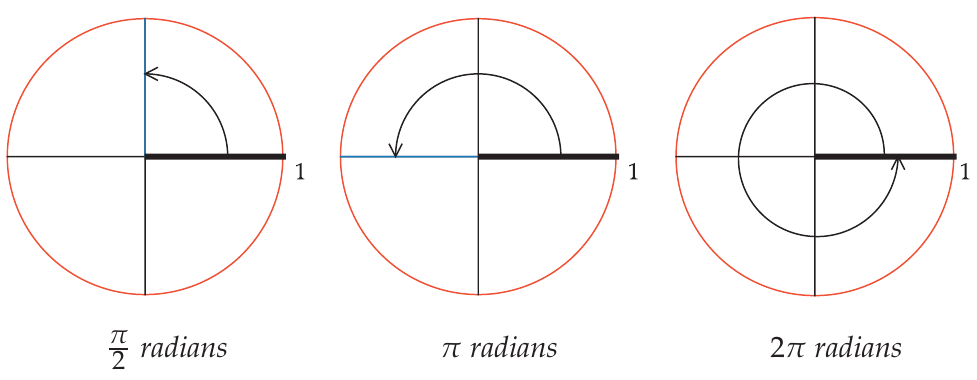
\includegraphics[scale=0.3]{intro/6.png}
\end{frame}
\begin{frame}
    \frametitle{Radians}
   \begin{block}{Degree to Radians}

    $$ 360^{\circ} = 2 \pi radians $$
    $$ 1 ^{\circ}  = \frac{2 \pi}{360} radians $$
    
   \end{block}
\end{frame}

\begin{frame}
    \frametitle{Arc Length}
    \begin{block}{length of a circular arc}
        If $0 < \theta \leq 2\pi$ , then a circular arc on the unit circle corresponding to $\theta$ radians
        has length $\theta$         
    \end{block}
\end{frame}

\begin{frame}
        \begin{figure}[h]    
            \begin{minipage}[b]{0.3\textwidth}
            \centering
            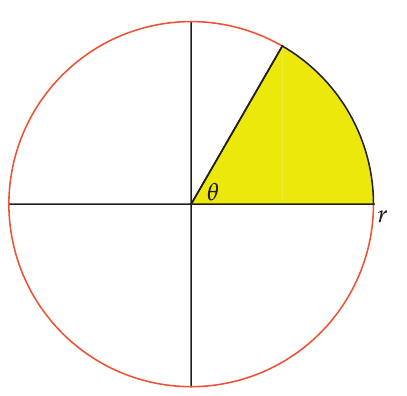
\includegraphics[scale=0.25]{intro/7.png}
            \caption{Area of slice}
        \end{minipage}
    \end{figure}
    \begin{block}{Area of slice}
        A slice with angle $\theta$ radians inside a circle with radius $r$ has area $\frac{1}{2} \theta r^{2}$ .
    \end{block}
\end{frame}
\begin{frame}
    \frametitle{Sine, Cosine and Tangent}
    \begin{figure}[h]    
        \begin{minipage}[b]{0.8\textwidth}
        \centering
        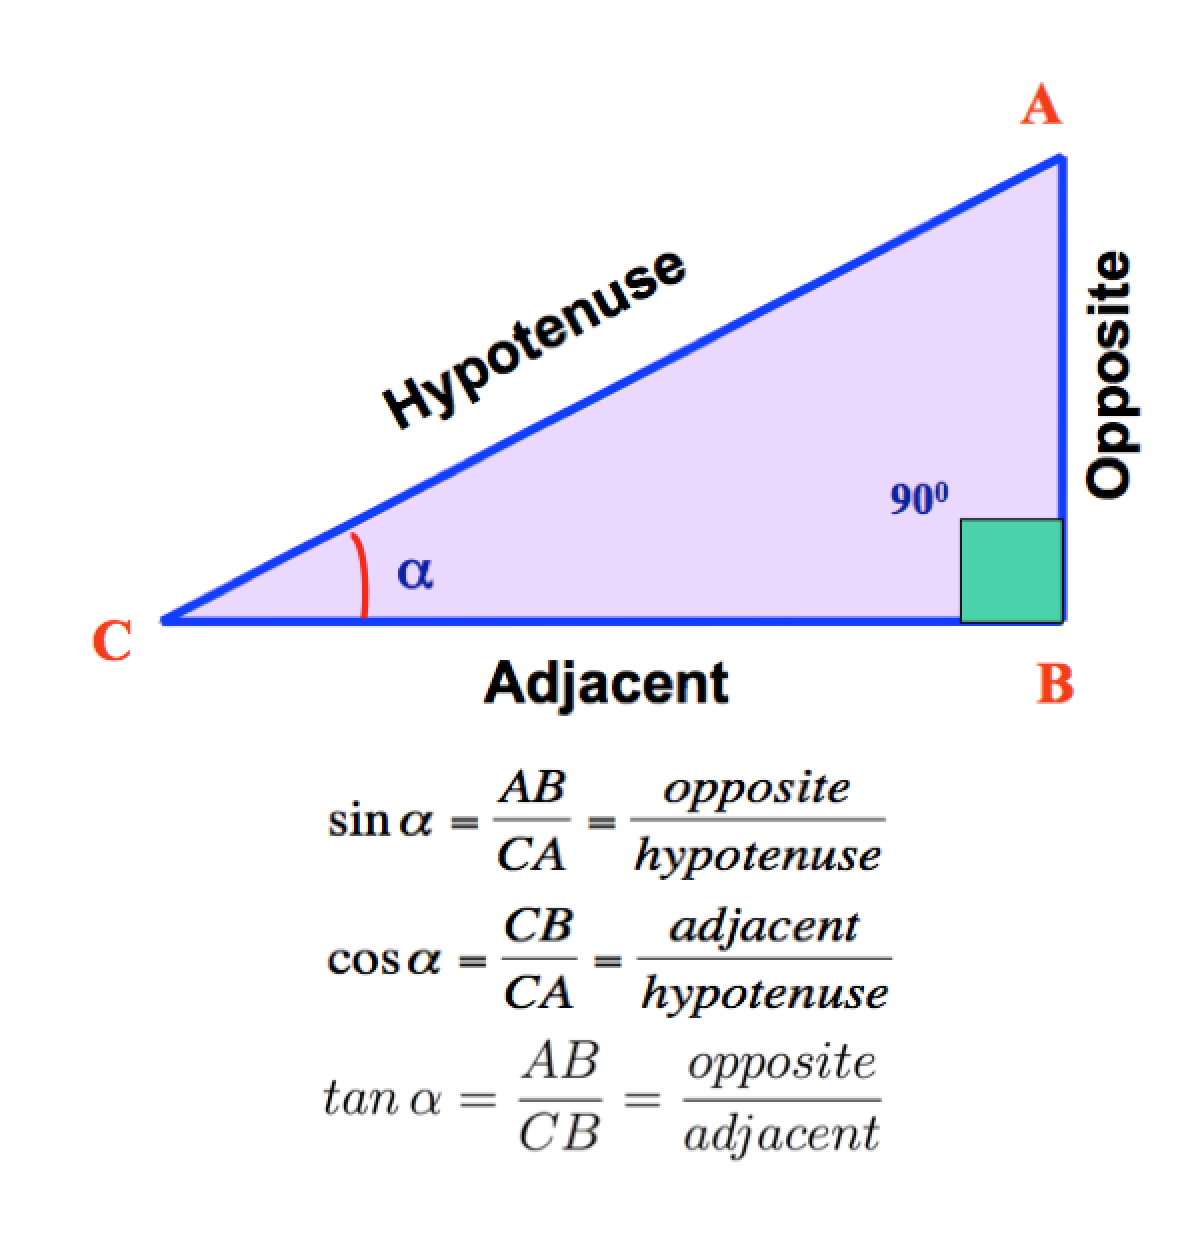
\includegraphics[scale=0.22]{intro/sine-cosine-tangent.png}
    \end{minipage}
\end{figure}
\end{frame}

\begin{frame}
    \frametitle{Unit Circle Co-ordinates}
    \begin{figure}[h]    
        \begin{minipage}[b]{0.8\textwidth}
        \centering
        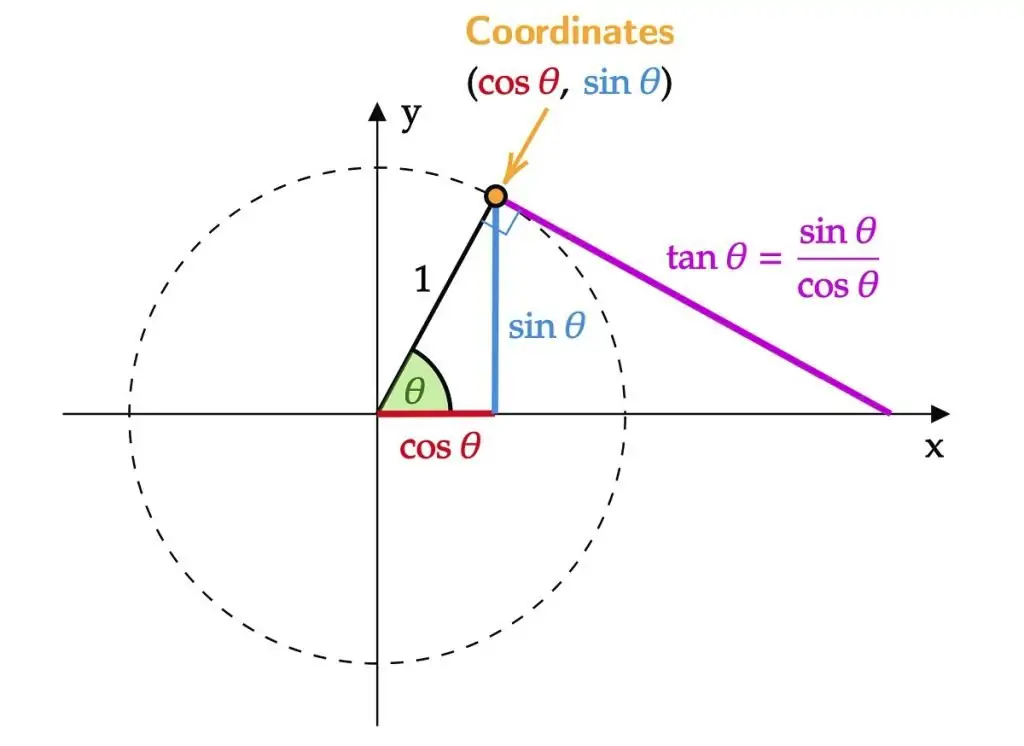
\includegraphics[scale=0.22]{intro/8.png}
    \end{minipage}
\end{figure}
\end{frame}


\section{Scalars and Vectors}
\begin{frame}
    \frametitle{Scalars vs Vectors}
    \begin{itemize}
        \item \textbf{Scalars:} Quantities described by a magnitude (e.g., temperature, mass).
        \item \textbf{Vectors:} Quantities described by both a magnitude and a direction (e.g., velocity, force).
    \end{itemize}
\end{frame}

\begin{frame}
    \frametitle{Vector Representation}
    \begin{itemize}
        \item Vectors can be represented graphically as arrows.
        \item The length of the arrow indicates the magnitude or it is shown as \(|\vec{v}|\).
        \item The direction of the arrow indicates the direction.
        \item Vectors are also denoted by a small arrow above the variable (e.g., \(\vec{v}\)).
    \end{itemize}
\end{frame}

\frame{
    \frametitle{Types of Vectors}
    \begin{itemize}
        \item \textbf{Zero Vector:} A vector with a magnitude of zero and no direction.
        \item \textbf{Unit Vector:} A vector with a magnitude of one, used to indicate direction and is given by \(\hat{v} = \frac{\vec{v}}{|\vec{v}|}\).
        \item \textbf{Position Vector:} A vector that represents the position of a point in space relative to an origin.
        \item \textbf{Collinear Vectors:} Vectors that lie along the same line or are parallel to each other.
        \item \textbf{Orthogonal Vectors:} Vectors that are perpendicular to each other.
        \item \textbf{Coplanar Vectors:} Vectors that lie in the same plane.
        \item \textbf{Negative Vectors:} Vectors that have the same magnitude as a given vector but point in the opposite direction.
        \item \textbf{Equal Vectors:} Vectors that have the same magnitude and direction.
        \item \textbf{Reciprocal Vectors:} Vectors having the same direction but their magnitudes are reciprocals of each other.
    \end{itemize}
}
\begin{frame}
    \frametitle{Position Vector}
    \begin{figure}
        \centering
        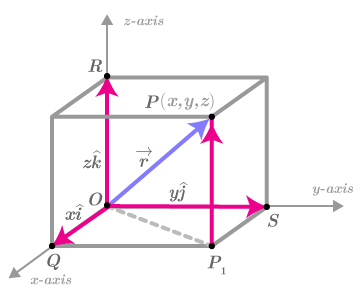
\includegraphics[width=0.4\textwidth]{position_vector.png}
        \caption{Position vector of a point in space}           
    \end{figure}
    
\end{frame}
\begin{frame}
    \frametitle{Position vector of a Point in Space}
    \begin{itemize}
        \item The position vector of a point \(P\) in space with coordinates \((x, y, z)\) is given by:
        \[
    \vec{OP} = x\hat{\imath} + y\hat{\jmath} + z\hat{k}
        \]
    where \(\hat{\imath}, \hat{\jmath}, \hat{k}\) are the unit vectors along the x, y, and z axes respectively. 

        \item The magnitude of the position vector is calculated as:
        \[
        |\vec{OP}| = \sqrt{x^2 + y^2 + z^2}
        \]
        \item The direction of the position vector is given by the angles it makes with the coordinate axes, which can be calculated using trigonometric functions.

    \end{itemize}
    
\end{frame}

\begin{frame}
    \frametitle{Direction Cosines}
    \begin{figure}
        \centering
        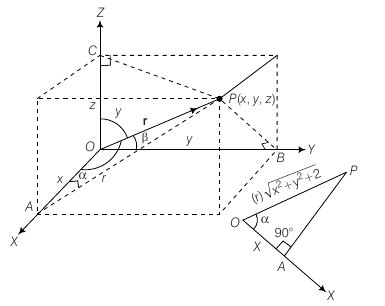
\includegraphics[width=0.6\textwidth]{direction_cosines.png}
        \caption{Direction cosines of a vector}
    \end{figure}
\end{frame}

\begin{frame}
    \frametitle{Direction Cosines}
    In $\delta OAP$ is right angled triangle 
    \[
    \cos \alpha = l = \frac{OA}{OP}  = \frac{x}{r} = \frac{x}{\sqrt{x^2 + y^2 + z^2}}
    \] 

    In $\delta OBP$ is right angled triangle
    \[
    \cos \beta = m = \frac{OB}{OP}  = \frac{y}{r} = \frac{y}{\sqrt{x^2 + y^2 + z^2}}
    \]

    In $\delta OCP$ is right angled triangle
    \[
    \cos \gamma = n = \frac{OC}{OP}  = \frac{z}{r} = \frac{z}{\sqrt{x^2 + y^2 + z^2}}
    \]
\end{frame}

\begin{frame}
    \frametitle{Direction Cosines}
    \begin{itemize}
        \item The direction cosines of a vector are the cosines of the angles that the vector makes with the coordinate axes.
        \item For a position vector \(\vec{OP}\), the direction cosines are given by:
        \[
        \cos \alpha = \frac{x}{|\vec{OP}|}, \quad \cos \beta = \frac{y}{|\vec{OP}|}, \quad \cos \gamma = \frac{z}{|\vec{OP}|}
        \]
        where \(\alpha, \beta, \gamma\) are the angles with the x, y, and z axes respectively.
        \item \(l^{2} + m^{2} + n^{2} = 1\)
    \end{itemize}
\end{frame}

\begin{frame}
    \frametitle{Direction Ratios}
    \begin{itemize}
        \item Direction ratios of \(\vec{OP}\) are any numbers proportional to \(x,y,z\); for the point \((x,y,z)\) itself they are \(x:y:z\).
        \item Relation with direction cosines: \(l=\frac{x}{r},\; m=\frac{y}{r},\; n=\frac{z}{r}\) where \(r=|\vec{OP}|=\sqrt{x^{2}+y^{2}+z^{2}}\); hence \(l:m:n = x:y:z\).
        \item Equivalently \(x = r l,\; y = r m,\; z = r n\). If you write \(l = kx,\; m = ky,\; n = kz\) then \(k = \tfrac{1}{r} = \tfrac{1}{|\vec{OP}|}\).
        \item In general, for any direction ratios \(a,b,c\): \(l = \frac{a}{\sqrt{a^{2}+b^{2}+c^{2}}},\; m = \frac{b}{\sqrt{a^{2}+b^{2}+c^{2}}},\; n = \frac{c}{\sqrt{a^{2}+b^{2}+c^{2}}}\).
    \end{itemize}
\end{frame}

\begin{frame}
\frametitle{Linear Combination of Vectors}
\begin{block}{Linear Combination}
A set of \(n\) vectors \(\vec{v_1}, \vec{v_2}, \ldots, \vec{v_n}\) can be combined linearly to form a new vector \(\vec{v}\):
\[
\vec{v} = c_1 \vec{v_1} + c_2 \vec{v_2} + \cdots + c_n \vec{v_n}
\]
where \(c_1, c_2, \ldots, c_n\) are scalars.
\end{block}
\end{frame}

\begin{frame}
    \frametitle{Relation between two Collinear Vectors}
    \begin{itemize}
        \item If two vectors \(\vec{a}\) and \(\vec{b}\) are collinear, then there exists a scalar \(k\) such that:
        \[
        \vec{b} = k \vec{a}
        \]
        where \(k\) is a non-zero scalar.
        \item Collinear vectors have the same or opposite direction.
        \item The scalar \(k\) can be positive or negative, indicating the direction of \(\vec{b}\) relative to \(\vec{a}\).
        \item If \(k > 0\), then \(\vec{b}\) points in the same direction as \(\vec{a}\). If \(k < 0\), then \(\vec{b}\) points in the opposite direction.
    \end{itemize}
\end{frame}

\begin{frame}
    \frametitle{Theorem of Coplanar Vectors}

    If three vectors \(\vec{a}, \vec{b}, \vec{c}\) are coplanar, then there exist scalars \(x, y, z\) such that:
    \[
    x \vec{a} + y \vec{b} + z \vec{c} = \vec{0}
    \]
    where not all of \(x, y, z\) are zero.      

    If two vectors \(\vec{a}, \vec{b}\) be two non-zero, non-collinear vectors, then any vector \(\vec{r}\) coplanar with \(\vec{a}\) and \(\vec{b}\) can be uniquely expressed as a linear combination of \(\vec{a}\) and \(\vec{b}\):
    \[
    \vec{r} = \lambda_1 \vec{a} + \lambda_2 \vec{b}
    \]
    for some scalars \(\lambda_1, \lambda_2\).

\end{frame}

\begin{frame}
\frametitle{Linear Dependence and Independence}
\begin{itemize}
    \item A set of vectors \(\{\vec{v_1}, \vec{v_2}, \ldots, \vec{v_n}\}\) is said to be linearly dependent if there exist scalars \(c_1, c_2, \ldots, c_n\), not all zero, such that:
    \[
    c_1 \vec{v_1} + c_2 \vec{v_2} + \cdots + c_n \vec{v_n} = \vec{0}
    \]
    \item If no such scalars exist, the vectors are linearly independent.
    \item Geometrically, linearly dependent vectors lie in the same line or plane, while independent vectors do not.
\end{itemize}                   
\end{frame}

\begin{frame}
    \frametitle{Product of Two Vectors}
    \begin{block}{Scalar product or Dot product}
        The scalar product (or dot product) of two vectors \(\vec{a}\) and \(\vec{b}\) is defined as:
        \[
        \vec{a} \cdot \vec{b} = |\vec{a}| |\vec{b}| \cos \theta
        \]
        where \(\theta\) is the angle between the two vectors.
        
    \end{block}
\end{frame}

\begin{frame}
    \frametitle{Geometric Interpretation of Dot Product}
    \begin{figure}
        \centering
        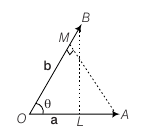
\includegraphics[width=0.4\textwidth]{dot_product.png}
        \caption{Geometric interpretation of the dot product}
    \end{figure}

\end{frame}

\begin{frame}
    \frametitle{Geometric Interpretation of Dot Product}
    From triangles \(\Delta OBL\) and \(\Delta OAM\):
    \begin{align*}
        OL &= OB \cos \theta \\
        OM &= OA \cos \theta  \\
        a \cdot b  &= |a| |b| \cos \theta = |a| proj_a b \\
        b \cdot a  &= |b| |a| \cos \theta = |b| proj_b a \\
    \end{align*}
\end{frame} 

\begin{frame}
\frametitle{Relevance of Dot Product: Physics}
The dot product is particularly useful in physics and engineering for calculating work done by a force. The work \(W\) done by a constant force \(\vec{F}\) acting on an object that undergoes a displacement \(\vec{d}\) is given by:
\[
W = \vec{F} \cdot \vec{d}
\]
\end{frame}

\begin{frame}
    \frametitle{Workdone by a Force}
    \begin{figure}
        \centering
        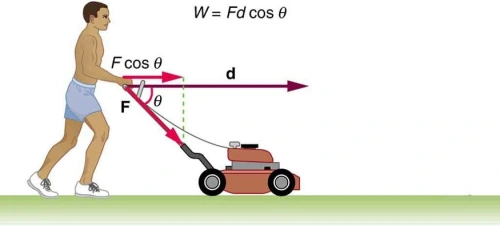
\includegraphics[width=0.8\linewidth]{force_dot.png}
    \end{figure}
\end{frame}

\begin{frame}
\frametitle{Force as a Scalar Product and the Role of Projection}
The work done by a force depends only on the component of the force in the direction of the displacement. If we write the unit vector in the direction of displacement as
\[
\hat{u}_{d} = \frac{\vec{d}}{|\vec{d}|},
\]
then the scalar (parallel) component of the force along the displacement is
\[
F_{\parallel} = \vec{F}\cdot\hat{u}_{d} = \frac{\vec{F}\cdot\vec{d}}{|\vec{d}|}.
\]
\end{frame} 

\begin{frame} 
    \frametitle{Force as a Scalar Product and the Role of Projection}
The work can therefore be written as the product of this scalar component and the magnitude of the displacement:
\[
W = F_{\parallel}\,|\vec{d}| = (\vec{F}\cdot\hat{u}_{d})\,|\vec{d}| = \vec{F}\cdot\vec{d}.
\]

The vector projection of \(\vec{F}\) onto \(\vec{d}\) (the part of the force that actually does the work) is
\[
\mathrm{proj}_{\vec{d}}\vec{F} = \left(\frac{\vec{F}\cdot\vec{d}}{|\vec{d}|^{2}}\right)\vec{d}.
\]
\end{frame} 

\begin{frame} 
    \frametitle{Workdone by a Force}
Key points:
\begin{itemize}
    \item Only the component of \(\vec{F}\) parallel to the displacement contributes to work; the perpendicular component does no work because its dot product with \(\vec{d}\) is zero.
    \item Writing work in terms of the projection makes the physical meaning clear: you are multiplying the displacement by the effective force acting along that displacement.
    \item Example: if an object is displaced horizontally by \(\vec{d}=d\hat{\imath}\) and \(\vec{F}=(F_x,F_y)\), then \(W=F_x d\) — only the horizontal component contributes.
\end{itemize}
\end{frame}
\begin{frame}
\frametitle{Relevance of Dot Product: Mathematics and Computer Science}
The dot product is also important in mathematics and computer science. Its applications include:
\begin{itemize}
    \item \textbf{Projection}: The dot product is used to project one vector onto another, which is useful in various algorithms.
    \item \textbf{Similarity}: In machine learning, the dot product is used to measure the similarity between two vectors, such as in document classification.
    \item \textbf{Graphics}: The dot product helps in determining the angle between vectors, which is essential in computer graphics for lighting and shading calculations.
\end{itemize}
\end{frame}
\begin{frame}
    \frametitle{Algebraic Properties of Dot Product}
    \begin{itemize}
        \item Commutative: \(a \cdot b = b \cdot a\)
        \item Distributive: \(a \cdot (b + c) = a \cdot b + a \cdot c\)
        \item Scalar multiplication: \((k a) \cdot b = k (a \cdot b)\)
    \end{itemize}
\end{frame}

\begin{frame}
    \frametitle{Vector Product or Cross Product}
    The vector product (or cross product) of two vectors \(\vec{a}\) and \(\vec{b}\) is defined as:
    \[
    \vec{a} \times \vec{b} = |\vec{a}| |\vec{b}| \sin \theta \, \hat{n}
    \]
    where \(\theta\) is the angle between the two vectors and \(\hat{n}\) is a unit vector perpendicular to the plane containing \(\vec{a}\) and \(\vec{b}\), following the right-hand rule.
\end{frame}

\begin{frame}
\frametitle{Geometric Interpretation of Cross Product}
\begin{figure}
    \centering
    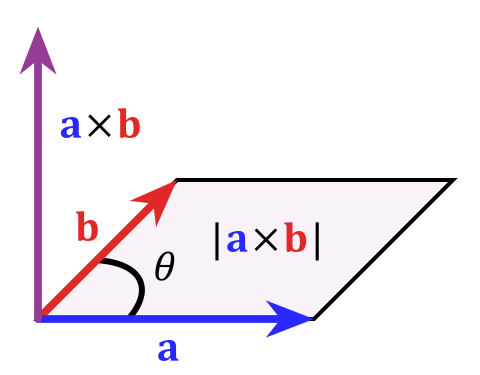
\includegraphics[width=0.4\textwidth]{cross_product.png}
    \caption{Geometric interpretation of the cross product}
\end{figure}
\end{frame} 

\begin{frame}
    \frametitle{Geometric Interpretation of Cross Product}
    The area of a parallelogram formed by two vectors \(\vec{a}\) and \(\vec{b}\) is given by the magnitude of their cross product:
    \[
    A = |\vec{a} \times \vec{b}|
    \]
    where \(\theta\) is the angle between the two vectors.

\end{frame}

\begin{frame}
    \frametitle{Algebraic Properties of Cross Product}
    \begin{itemize}
        \item Anticommutative: \(\vec{a} \times \vec{b} = -(\vec{b} \times \vec{a})\)
        \item Distributive: \(\vec{a} \times (\vec{b} + \vec{c}) = \vec{a} \times \vec{b} + \vec{a} \times \vec{c}\)
        \item Scalar multiplication: \((k \vec{a}) \times \vec{b} = k (\vec{a} \times \vec{b})\)
        \item The cross product of two parallel vectors is zero: if \(\vec{a}\) and \(\vec{b}\) are parallel, then \(\vec{a} \times \vec{b} = 0\).
        \item The magnitude of the cross product can be interpreted as the area of the parallelogram formed by the two vectors: \(|\vec{a} \times \vec{b}| = |\vec{a}| |\vec{b}| \sin \theta\).
    \end{itemize}
\end{frame}

\begin{frame}
    \frametitle{Relevance of Cross Product: Physics}
    The cross product is particularly useful in physics and engineering for determining a vector that is perpendicular to a plane defined by two other vectors. This has applications in:
    \begin{itemize}
        \item \textbf{Torque}: The torque \(\vec{\tau}\) exerted by a force \(\vec{F}\) applied at a position \(\vec{r}\) is given by the cross product:
        \[
        \vec{\tau} = \vec{r} \times \vec{F}
        \]
        \item \textbf{Angular Momentum}: The angular momentum \(\vec{L}\) of a particle is given by:
        \[
        \vec{L} = \vec{r} \times \vec{p}
        \]
        where \(\vec{p}\) is the linear momentum.
        \item \textbf{Magnetic Force}: The force \(\vec{F}\) on a charged particle moving with velocity \(\vec{v}\) in a magnetic field \(\vec{B}\) is given by:
        \[
        \vec{F} = q \vec{v} \times \vec{B}
        \]
    \end{itemize}
\end{frame}

\begin{frame}
    \frametitle{Force and Torque} 
    \begin{figure}
        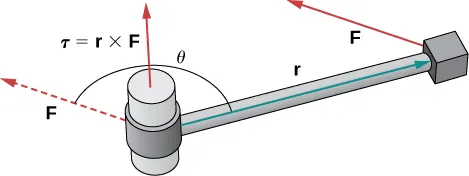
\includegraphics[width=0.8\linewidth]{torque_force.png}
    \end{figure}
\end{frame}

\begin{frame}
    \frametitle{Relevance of Cross Product: Mathematics and Computer Graphics}
    The cross product is also important in mathematics and computer graphics. Its applications include:
    \begin{itemize}
        \item \textbf{Normal Vectors}: In computer graphics, the cross product is used to find normal vectors to surfaces, which are essential for lighting calculations.
        \item \textbf{3D Rotations}: The cross product helps in determining the axis of rotation and the angle of rotation in 3D space.
        \item \textbf{Area Calculation}: The magnitude of the cross product of two vectors can be used to find the area of the parallelogram formed by the vectors.
    \end{itemize}
\end{frame}

\begin{frame}
    \frametitle{Algebraic properties of Vector Product}
    \begin{itemize}
        \item Anticommutative: \(\vec{a} \times \vec{b} = -(\vec{b} \times \vec{a})\)
        \item Distributive: \(\vec{a} \times (\vec{b} + \vec{c}) = \vec{a} \times \vec{b} + \vec{a} \times \vec{c}\)
        \item Scalar multiplication: \((k \vec{a}) \times \vec{b} = k (\vec{a} \times \vec{b})\)
        \item The cross product of two parallel vectors is zero: if \(\vec{a}\) and \(\vec{b}\) are parallel, then \(\vec{a} \times \vec{b} = 0\).
        \item The magnitude of the cross product can be interpreted as the area of the parallelogram formed by the two vectors: \(|\vec{a} \times \vec{b}| = |\vec{a}| |\vec{b}| \sin \theta\).
    \end{itemize}
\end{frame}

\begin{frame}
\frametitle{Vector Product in terms of Components}
The cross product of two vectors \(\vec{a} = (a_1, a_2, a_3)\) and \(\vec{b} = (b_1, b_2, b_3)\) can be expressed in terms of its components as follows:
\[
\vec{a} \times \vec{b} = \begin{vmatrix}
\hat{i} & \hat{j} & \hat{k} \\
a_1 & a_2 & a_3 \\
b_1 & b_2 & b_3
\end{vmatrix}
= \hat{i}(a_2b_3 - a_3b_2) - \hat{j}(a_1b_3 - a_3b_1) + \hat{k}(a_1b_2 - a_2b_1)
\]
\end{frame}

\begin{frame}
\frametitle{Vector Normal to the plane of Two given Vectors}
If \(\vec{a}\) and \(\vec{b}\) are two non-parallel, non-zero vectors in \(\mathbb{R}^3\) and let \(\theta\) be the angle between them, then 
\begin{align*}
    \vec{a} \times \vec{b} &= |\vec{a}| |\vec{b}| \sin \theta \, \hat{n} \\
    \hat{n} &= \frac{\vec{a} \times \vec{b}}{|\vec{a} \times \vec{b}|}
\end{align*}             
\end{frame}





\section{3D Geometry}
\label{sec:3d_geometry}

\begin{frame}
    \frametitle{3D coordinates}
    \begin{figure}
        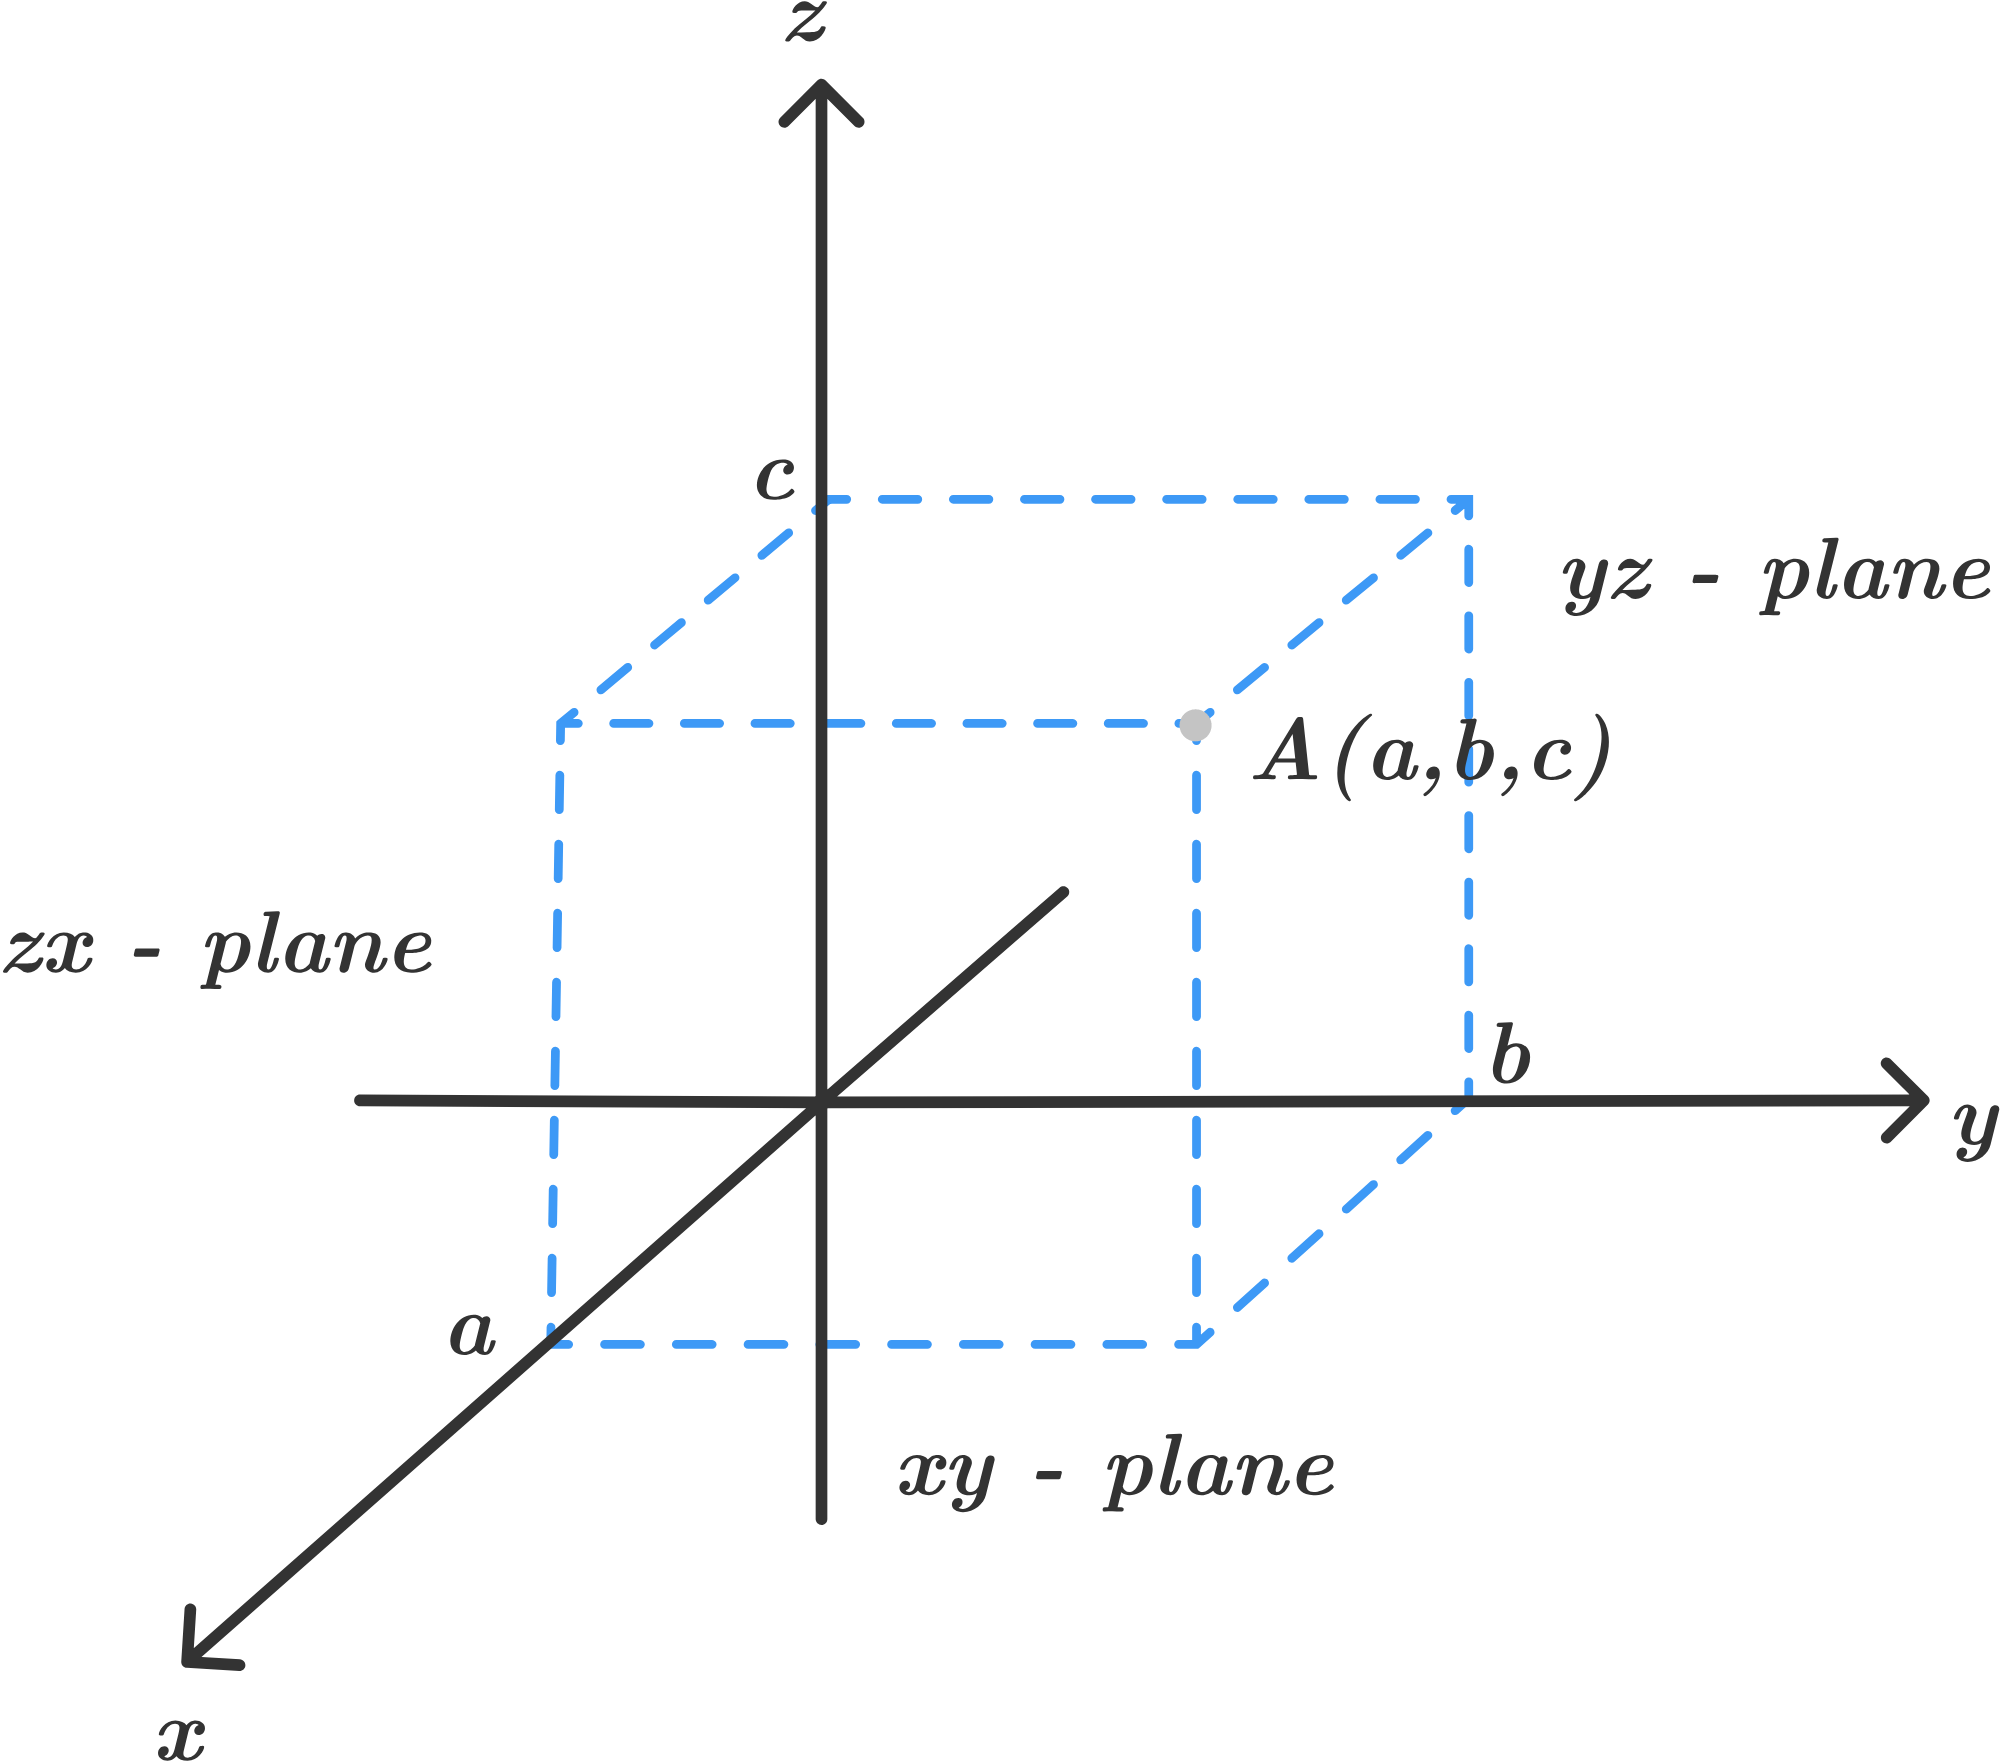
\includegraphics[scale=0.1]{3d_geometry/co_ordinate_plane.png}
        \caption{3D Coordinate Plane}
    \end{figure}
\end{frame}

\begin{frame}
    \frametitle{3D Coordinate System}
    \begin{itemize}
        \item The 3D coordinate system is defined by three mutually perpendicular axes: the x-axis, y-axis, and z-axis.
        \item A point in 3D space is represented by its coordinates \(P(x, y, z)\).
        \item The position vector of a point \(P\) in 3D space is given by:
        \[
        \vec{OP} = x\hat{\imath} + y\hat{\jmath} + z\hat{k}
        \]
    \end{itemize}       
\end{frame}

\begin{frame}
    \frametitle{Shifting the Origin}
    \begin{block}{Translation of Axes}
        Shifting the origin  to another point without changing the direction of axes is called \textbf{translation}.
    \end{block}
   Let the origin \(O\) be shifted to a new point \(O'\) with coordinates \(O'(x_0, y_0, z_0)\). The position vector of a point \(P(x,y,z)\) with respect to the new origin \(O'\) given by :
    \[
        \vec{O'P} = (x - x_0)\hat{\imath} + (y - y_0)\hat{\jmath} + (z - z_0)\hat{k}
    \]
\end{frame}

\begin{frame}
\frametitle{Distance Formula in 3D}
\begin{figure}
    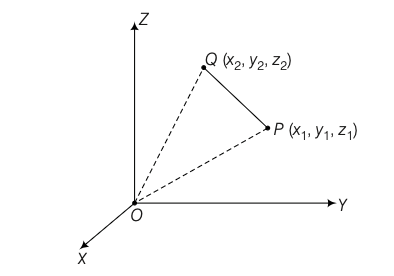
\includegraphics[scale=0.1]{3d_geometry/distance.png}
    \caption{Distance Formula in 3D}
\end{figure}
Let \(OP = x \hat{\imath} + y \hat{\jmath} + z \hat{k}\)  and \(OQ = x' \hat{\imath} + y' \hat{\jmath} + z' \hat{k}\) be two points in 3D space. The distance \(d\) between points \(P\) and \(Q\) is given by the formula:
\begin{align*}
    \vec{OQ} &= \vec{OP} + \vec{PQ} \\
    \vec{PQ} &= \vec{OQ} - \vec{OP} \\
    d &= |\vec{PQ}| = \sqrt{(x' - x)^2 + (y' - y)^2 + (z' - z)^2}
\end{align*}
\end{frame}

\begin{frame}
    \frametitle{Section Formula}
    \begin{figure}
        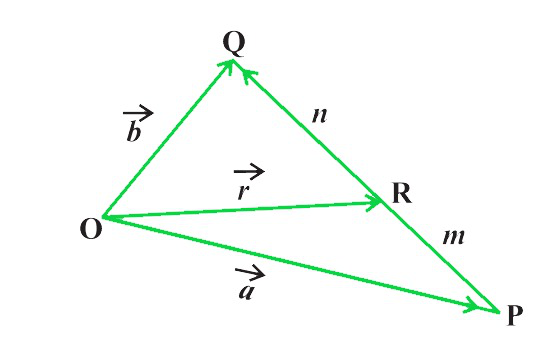
\includegraphics[scale=0.3]{3d_geometry/section.png}
        \caption{Section Formula in 2D}
    \end{figure} 
\end{frame}


\begin{frame}
    \begin{block}{Section Formula in 3D}
    Let \(P(x_1, y_1, z_1)\) and \(Q(x_2, y_2, z_2)\) be two points in 3D space with position vectors \( \vec{\mathbf{r}_1} \), \( \vec{\mathbf{r}_2} \) respectively. If a point \(R\) divides the line segment \(PQ\) in the ratio \(m:n\), then the position vector of point \(R\) is given by:
    \[
    \vec{\mathbf{r}} = \frac{m\vec{\mathbf{r}_2} + n\vec{\mathbf{r}_1}}{m+n}
    \]
    \end{block}
\end{frame}

\begin{frame}
    \frametitle{Proof of Section Formula}
    \begin{block}{Given}
    Point \(R\) divides line segment \(PQ\) internally in the ratio \(m:n\), where \(P\) and \(Q\) have position vectors \(\vec{\mathbf{a}}\) and \(\vec{\mathbf{b}}\) respectively.
    \end{block}
    
    \begin{block}{To Prove}
    The position vector of \(R\) is \(\vec{\mathbf{r}} = \frac{m\vec{\mathbf{b}} + n\vec{\mathbf{a}}}{m+n}\)
    \end{block}
    
    \begin{block}{Proof}
    Since \(R\) divides \(PQ\) in ratio \(m:n\):
    \begin{align}
        \frac{|\vec{PR}|}{|\vec{RQ}|} &= \frac{m}{n} \\
        \text{Since } \vec{PR} \text{ and } \vec{RQ} \text{ are collinear:} \quad \vec{PR} &= \frac{m}{n}\vec{RQ}
    \end{align}
    \end{block}
\end{frame}

\begin{frame}
    \frametitle{Proof of Section Formula (continued)}
    
    From vector addition: \(\vec{PR} + \vec{RQ} = \vec{PQ}\)
    
    Substituting \(\vec{PR} = \frac{m}{n}\vec{RQ}\):
    \begin{align}
        \frac{m}{n}\vec{RQ} + \vec{RQ} &= \vec{PQ} \\
        \vec{RQ}\left(\frac{m}{n} + 1\right) &= \vec{PQ} \\
        \vec{RQ} &= \frac{n}{m+n}\vec{PQ}
    \end{align}

\end{frame}


\begin{frame}
 
    Since \(\vec{PQ} = \vec{\mathbf{b}} - \vec{\mathbf{a}}\) and \(\vec{RQ} = \vec{\mathbf{b}} - \vec{\mathbf{r}}\):
    \begin{align}
        \vec{\mathbf{b}} - \vec{\mathbf{r}} &= \frac{n}{m+n}(\vec{\mathbf{b}} - \vec{\mathbf{a}}) \\
        \vec{\mathbf{r}} &= \vec{\mathbf{b}} - \frac{n}{m+n}(\vec{\mathbf{b}} - \vec{\mathbf{a}}) \\
        \vec{\mathbf{r}} &= \frac{m\vec{\mathbf{b}} + n\vec{\mathbf{a}}}{m+n}
    \end{align}
  
\end{frame}

\begin{frame}
\frametitle{Direction Ratios}
\begin{block}{Direction Ratios}
    The direction ratios of a line are any three numbers that are proportional to the direction cosines of the line. If a line has direction cosines \(l, m, n\), then its direction ratios can be represented as \(a, b, c\) such that:
    \begin{align*}
        l = \frac{a}{\sqrt{a^2 + b^2 + c^2}}, \quad m = \frac{b}{\sqrt{a^2 + b^2 + c^2}}, \quad n = \frac{c}{\sqrt{a^2 + b^2 + c^2}} 
        l &= k a \\
        m &= k b \\
        n &= k c
    \end{align*}
\end{block} 
\begin{itemize}
    \item It is evident that the direction ratios are not unique, as they can be scaled by any non-zero constant \(k\).
    \item However, the ratios \(a:b:c\) remain constant regardless of the scaling
\end{itemize}
\end{frame}

\begin{frame}
    \frametitle{Equation of a Line passing through a given point and parallel to a given vector}
    \begin{figure}
        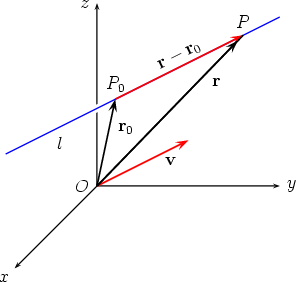
\includegraphics[scale=0.4]{3d_geometry/line_parallel_vector.png}
        \caption{Line in 3D space}
    \end{figure}
\end{frame}


\begin{frame}
\frametitle{Equation of a Line passing through a given point and parallel to a given vector}
    Let \(P_{0}(x_0, y_0, z_0)\) be a point on the line and \(P_{1}(x_1, y_1, z_1)\) be another point on the line. The direction vector of the line can be defined as \(\vec{P_{0}P_{1}} = \vec{r}_1 - \vec{r}_0\), where \(\vec{r}_0\) and \(\vec{r}_1\) are the position vectors of \(P_0\) and \(P_1\) respectively. The vector equation of the line can be expressed as:
    \[
    \vec{r} - \vec{r_0} = t\vec{v}
    \]
    where \(t\) is a scalar parameter. 
\end{frame}

\begin{frame}
    \frametitle{Direction Cosines vs. Direction Ratios: The Intuition}
    \begin{itemize}
        \item \textbf{Direction Cosines (DCs):} A unique, standardized recipe. They tell you how much to travel along each axis to move exactly one unit along the line. The sum of their squares is always 1: \(l^2 + m^2 + n^2 = 1\).
        \item \textbf{Direction Ratios (DRs):} A flexible, proportional recipe. They tell you the ratio of movement along the axes. For every 'a' units in x, you move 'b' units in y and 'c' units in z. They are not unique; any scalar multiple represents the same direction.
    \end{itemize}
\end{frame}

\begin{frame}
    \frametitle{Direction Cosines (DCs): Mathematical Definition}
    Let a vector \(\vec{v}\) make angles \(\alpha, \beta, \gamma\) with the positive X, Y, and Z axes.
    \begin{itemize}
        \item \(l = \cos(\alpha)\)
        \item \(m = \cos(\beta)\)
        \item \(n = \cos(\gamma)\)
    \end{itemize}
    \begin{figure}
        \includegraphics[width=0.6\textwidth]{direction_cosine_angles.png}
        \caption{Angles for Direction Cosines}
    \end{figure}
    For a vector \(\vec{v} = (x, y, z)\) with magnitude \(|\vec{v}| = \sqrt{x^2 + y^2 + z^2}\):
    \[ l = \frac{x}{|\vec{v}|}, \quad m = \frac{y}{|\vec{v}|}, \quad n = \frac{z}{|\vec{v}|} \]
    A key property is that \(l^2 + m^2 + n^2 = 1\).
\end{frame}

\begin{frame}
    \frametitle{Converting Direction Ratios to Direction Cosines}
    If you have direction ratios \((a, b, c)\), you can find the direction cosines \((l, m, n)\) by normalizing them:
    \[ l = \frac{a}{\sqrt{a^2 + b^2 + c^2}} \]
    \[ m = \frac{b}{\sqrt{a^2 + b^2 + c^2}} \]
    \[ n = \frac{c}{\sqrt{a^2 + b^2 + c^2}} \]
    This process creates a unit vector, which is what the direction cosines represent.
\end{frame}

\begin{frame}
    \frametitle{Equation of a Line: Two-Point Form}
    Given two points on the line, \(A(x_1, y_1, z_1)\) and \(B(x_2, y_2, z_2)\).
    \begin{block}{Vector Form}
        Let the position vectors of A and B be \(\vec{a}\) and \(\vec{b}\). The direction vector is \(\vec{d} = \vec{b} - \vec{a}\). The equation of the line is:
        \[ \vec{r} = \vec{a} + \lambda(\vec{b} - \vec{a}) \]
    \end{block}
    \begin{block}{Cartesian Form}
        The direction ratios are \((x_2 - x_1, y_2 - y_1, z_2 - z_1)\). The equation is:
        \[ \frac{x - x_1}{x_2 - x_1} = \frac{y - y_1}{y_2 - y_1} = \frac{z - z_1}{z_2 - z_1} \]
    \end{block}
\end{frame}






\end{document}
